\documentclass[jair,twoside,11pt,theapa]{article}
\usepackage{jair, theapa, rawfonts}
\usepackage{times}
\usepackage{latexsym}
\usepackage{amsmath}
\usepackage{bbm}
\usepackage{multirow}
\usepackage{url}
\usepackage{color}
\usepackage{epsfig,url,algorithm,algorithmic,multirow}
%\usepackage{microtype}
\usepackage{amssymb}


\DeclareMathOperator*{\argmax}{arg\,max}

\usepackage{booktabs}
\usepackage{graphicx}
\usepackage{varwidth}

\renewcommand{\paragraph}[1]{\noindent\textbf{#1.}}

\newcommand{\squishlist}{
 \begin{list}{}
  { \setlength{\itemsep}{0pt}
     \setlength{\parsep}{3pt}
     \setlength{\topsep}{3pt}
     \setlength{\partopsep}{0pt}
     \setlength{\leftmargin}{3em}
     \setlength{\labelwidth}{1em}
     \setlength{\labelsep}{0.5em} } }

\jairheading{x}{year}{x-xx}{m/yy}{m/yy}
\ShortHeadings{Machine Reading  with High Volume  Memory} 
{Nakashole \& Mitchell}
\firstpageno{1}

\begin{document}

\title{Machine Reading   with  High Volume  Memory}

\author{\name  Nakashole \email ndapa@cs.cmu.edu \\
       \addr Carnegie Mellon University\\
       5000 Forbes Avenue \\
		Pittsburgh, PA, 15213
       \AND
       \name Tom M Mitchell\email tom.mitchell@cs.cmu.edu \\
       \addr Carnegie Mellon University\\
       5000 Forbes Avenue \\
		Pittsburgh, PA, 15213
       }
       
%\author{}

% For research notes, remove the comment character in the line below.
% \researchnote

\maketitle


\begin{abstract}
In artificial intelligence, the goal of machine reading is to develop systems that automatically understand natural language text.   
A key challenge in machine reading  arises from a significant amount information not being explicitly stated  but instead  implied by the text in combination with  background knowledge. This means that machine reading methods that rely on  context alone are inherently limited in their understanding capabilities. In this paper, we advocate and  study machine reading methods that incorporate  comprehensive, high volume world knowledge in their inference mechanisms.
To this end, we  have developed methods for sentence level machine reading  that make use of  background knowledge.  
The first method addresses prepositional phrase attachment ambiguity. Our  method  uses  background knowledge within a semi-supervised machine learning algorithm that learns from both labeled and unlabeled data. The approach produced state-of-the-art results on two datasets and  performed significantly better than  a widely used dependency parser. The second method aims to extract relationships from compound nouns.  We have developed a  knowledge-aware method for compound noun analysis, our experiments show that it accurately extracts beliefs from compound nouns.

\end{abstract}

\section{Introduction}
\label{Introduction}
Artificial intelligence  researchers have long sought to build systems capable of automatically reading  understanding  natural language text -- machine reading systems. A computer program is said to understand 
language if it responds appropriately to instructions in natural language. For example, if the task is to read a piece of text and answer questions about it, then a program understands if it outputs the correct answers.  If the task is to translate from one language to another, the program understands if it correctly  translates from the source language to the target language. And if the task is to extract information about which drugs treats which physiological conditions,  the program understands if it finds the correct pairs of drugs and physiological conditions.

Machine reading methods can be characterized based on their awareness of  world knowledge.
On one extreme end, there are methods that  are oblivious to background knowledge, \textit{reading from scratch methods}. On the opposite  end, there are  knowledge-intensive methods that incorporate comprehensive, high volume world knowledge in their inference mechanisms, \textit{reading with high volume memory}. A key challenge in language understanding is that some information is not explicitly stated in text but it is implied by the text in combination with  background knowledge. For example, if the text states that Alice left a restaurant after a good meal, one can infer, with some probability, that she paid the bill and left a tip. In reference resolution, consider the sentence ``The bee landed on the flower because it wanted pollen.''  If we know that  bees feed on pollen, we can correctly determine that ``it''   refers to the bee and not the flower.  In negation detection, consider the sentence:  ``Things would be different if Microsoft was headquartered in Texas.''  From this sentence alone, a machine reading program might incorrectly extract a belief that  Microsoft is headquartered in Texas. But from the prior knowledge that Microsoft was never headquartered in Texas, we might be able to better detect the negation, in addition to the syntactic cues such as ``if''. Thus, inference over prior knowledge is crucial to  text understanding. When humans read, this kind of inference is natural.  Studies of brain scans of people's brains while reading fiction have found that readers mentally simulate each new situation encountered in a story\cite{conf/emnlp/WehbeVKM14}. Details about actions and
sensation are captured from the text and integrated with personal knowledge from past experiences. 
%And therefore,  machine reading methods that read from scratch are inherently limited in what they can understand. 

 In this paper, we  study machine reading methods that leverage a  high volume  memory  of beliefs about the world. 
In particular, we have developed two methods for sentence level machine reading  that make use of  background knowledge:
\begin{enumerate}

\item The first method addresses  a difficult case of syntactic ambiguity caused by prepositions. Prepositions  such as ``in'', ``at'', and ``for" express important details about the where, when, and why of relations and events. However, prepositions are major source of syntactic ambiguity and still pose problems in language analysis. In particular, they cause the problem of prepositional phrase attachment ambiguity, which  arises in cases such as  ``she caught the butterfly with the spots" vs. ``she caught the butterfly with the net". In the first case,  the preposition ``with''  modifies the verb ``caught", while in the second case, ``with" modifies the noun ``butterfly". Disambiguating  these two attachments requires knowing that butterflies can have spots,  and that a net is an instrument that can be used for catching. Our  approach  uses this type of knowledge within a semi-supervised machine learning algorithm that learns from both labeled and unlabeled data. The approach produced state-of-the-art results on two datasets and  performed significantly better than  a syntactic parser that most people use in their natural language processing pipelines. 
 
 \item The second method that exploits background knowledge for language understanding extracts relationships from compound nouns such as  ``pro-choice Democratic gubernatorial  candidate  James Florio'', or  ``White  House spokesman Marlin Fitzwater''.  Compound nouns  
contain a number of challenging compositional phenomena, including implicit relations. Compound nouns mostly consist of adjectives and nouns, they do not contain verbs. That means there are often no lexical commonalities even across compound nouns that express the same relations,  making it difficult to extract beliefs from them. On the other hand, beliefs such as a person's job title, nationality, or stance on a political issue are often expressed using compound nouns. We have developed a  knowledge-aware method for compound noun analysis which accurately extracts relationships from compound nouns.
 \end{enumerate}
 
% 
% We highlight the  challenges and  report experimental results for our  machine reading methods that have access to background knowledge which we compare to results of methods that read from scratch.

\subsection{ High Volume Memory}
By high volume memory we mean storage capable of storing and retrieving   comprehensive world
knowledge akin to the breadth of  world knowledge   adult human brains have a grasp of. Such a high volume memory, therefore,  contains beliefs
about the world, the objects in it,   their properties, and  approximate confidence scores for beliefs held.

\paragraph{Knowledge Bases} Towards realizing high volume memories of world knowledge, knowledge base construction projects have accumulated large amounts of beliefs about real world entities  \cite{MitchellCHTBCMG15,suchanek2007yago,Bollacker2008}. Large-scale knowledge bases are populated by applying machine reading methods to  web corpora.  For example, the  Never-Ending
Language Learner (NELL)  system  has been learning to read the web 24 hours/day for over several years. However,  current machine reading methods have been successful at populating knowledge bases  by means of pattern detection--- a shallow way of machine reading which leverages the redundancy of large corpora to capture language patterns. However, machine readers still lack the ability to fully understand  language. In the pursuit of the much harder goal of language comprehension, knowledge bases present an opportunity for a virtuous circle:  the accumulated knowledge can be used to improve machine readers; in turn, advanced reading methods can be used to populate knowledge bases with beliefs expressed using complex and potentially ambiguous language. There has been little work on making use of knowledge bases in machine reading. \cite{conf/acl/KrishnamurthyM14} introduced a method for  training a joint syntactic
and semantic parser. Their parser makes use of a knowledge base to produce  logical forms containing knowledge base predicates. However, their use of the knowledge base is limited to unary predicates  to determine  semantic types of concepts. In contrast,  in this paper we make extensive use of  a   knowledge base augmented by linguistic resources and corpus statistics  as the content  of a high volume memory  that our knowledge-aware methods have access to at inference time.

\paragraph{Neural Networks with Long-Term Memory}  Recent years have seen wide use of neural network models  for language understanding. For example neural networks have been applied to the task of answering queries about short stories,  and to the task of language modeling where the task is to predict the next word(s) in a text sequence given the previous
words \cite{MikolovKBCK10,SundermeyerSN12,WestonCB14,sukhbaatar2015end}. These tasks are  treated as instances of sequence processing, where the sequence consists of sentences or   in the case of language modeling the  sequence consists of  words. A number of studies have explored neural networks that model  long-term  structure in sequences
using recurrent neural networks (RNNs) including Long short-term memory  (LSTMs ) \cite{hochreiter1997long,atkeson1995memory,graves2013generating}. However, the memory in these models is the state
of the network which is encoded using latent states and weights. This memory is therefore typically  too small  and  not structured enough
to  remember facts from the past since background knowledge is compressed into dense vectors.  Additionally, in neural approaches, to retrieve relevant memories, 
smooth lookups are performed, whereby each memory is scored for its relevance, this may not scale well to the case where a larger memory is required. A notable exception in this line of work  is the work of \cite{WestonCB14} which introduced  memory networks  combining RNN inference with a long-term memory. They applied their models to the  task of answering queries about short stories. However background knowledge in this work is raw text from the story  as opposed to high volume world knowledge.  While they also performed an experiment on a question answering setting with   background knowledge consisting  of 14M  statements stored as (subject, relation, object) triples, this setting  is not a machine reading task but  an information retrieval task since there was no reading required to answer the questions, but only look up to find the triples most relevant to  the question.



\subsection{Contributions}
Our main contributions are as follows:
 
\textit{1)~Machine Reading   with  High Volume  Memory:}  We describe the problem of machine reading
with high volume memory. While the problem of machine reading has attracted a lot of attention in recent years,
there's been very little work on machine reading with high volume memory. This setting is unique and raises new questions which we study within the context of two problems: prepositional phrase attachment, and compound noun relation extraction. 
 
\textit{2)~Prepositional Phrase Attachment: }  We present  a knowledge-aware method for prepositional phrase attachment.
Previous  methods largely rely on  corpus statistics. Our approach  draws upon 
 diverse sources of background knowledge, leading to performance improvements. 
In addition to training on labeled  data, we also make use of a large amount of unlabeled data. This enhances our method's ability to generalize to diverse data sets. 
In addition to the standard Wall Street Journal corpus (WSJ)~\cite{Ratnaparkhi1994}, we labeled two new datasets for testing purposes, one from Wikipedia (WKP), and another from the  New York Times Corpus (NYTC). We make  these datasets freely available for future research.  In addition, we have applied our  model to over 4 million 5-tuples of the form $\{n0, v, n1, p, n2\}$, and we also make this dataset  available\footnote{http://rtw.ml.cmu.edu/resources/ppa}.
Although this work was first published in 

\textit{3)~Compound Noun Analysis: }  We introduce a knowledge-aware method for extracting relations from compound nouns. We collected over 2 million compound nouns from which we learned fine-grained semantic type sequences that express relations from the NELL knowledge base. Our experiments show that the accuracy of relations extracted in this manner is quite high.


\subsection{Organization}
The rest of the paper is organized as follows. We begin by presenting our knowledge-aware methods for machine reading.  Section \ref{ppa} presents our knowledge-aware approach to 
prepositional phrase attachment ambiguity. Section \ref{nominals} introduces our  knowledge-aware approach to relation extraction from compound nouns. Lastly, Section \ref{conclusions} provides concluding remarks and future directions.

 
\section{Prepositional Phrase Attachment}\label{ppa}
Prepositional phrases (PPs)   express crucial information that  information extraction  methods need to extract.
 % comprehensively extract facts. 
 However, PPs are a major source of  syntactic  ambiguity. In this paper, we propose to use semantic knowledge to  improve PP attachment disambiguation. 
 PPs such as  ``in", ``at", and ``for" express details about the  \textit{where, when,} and \textit{why}  of  relations and events. PPs   also state  attributes of nouns. 

\begin{figure}[t]

\centering

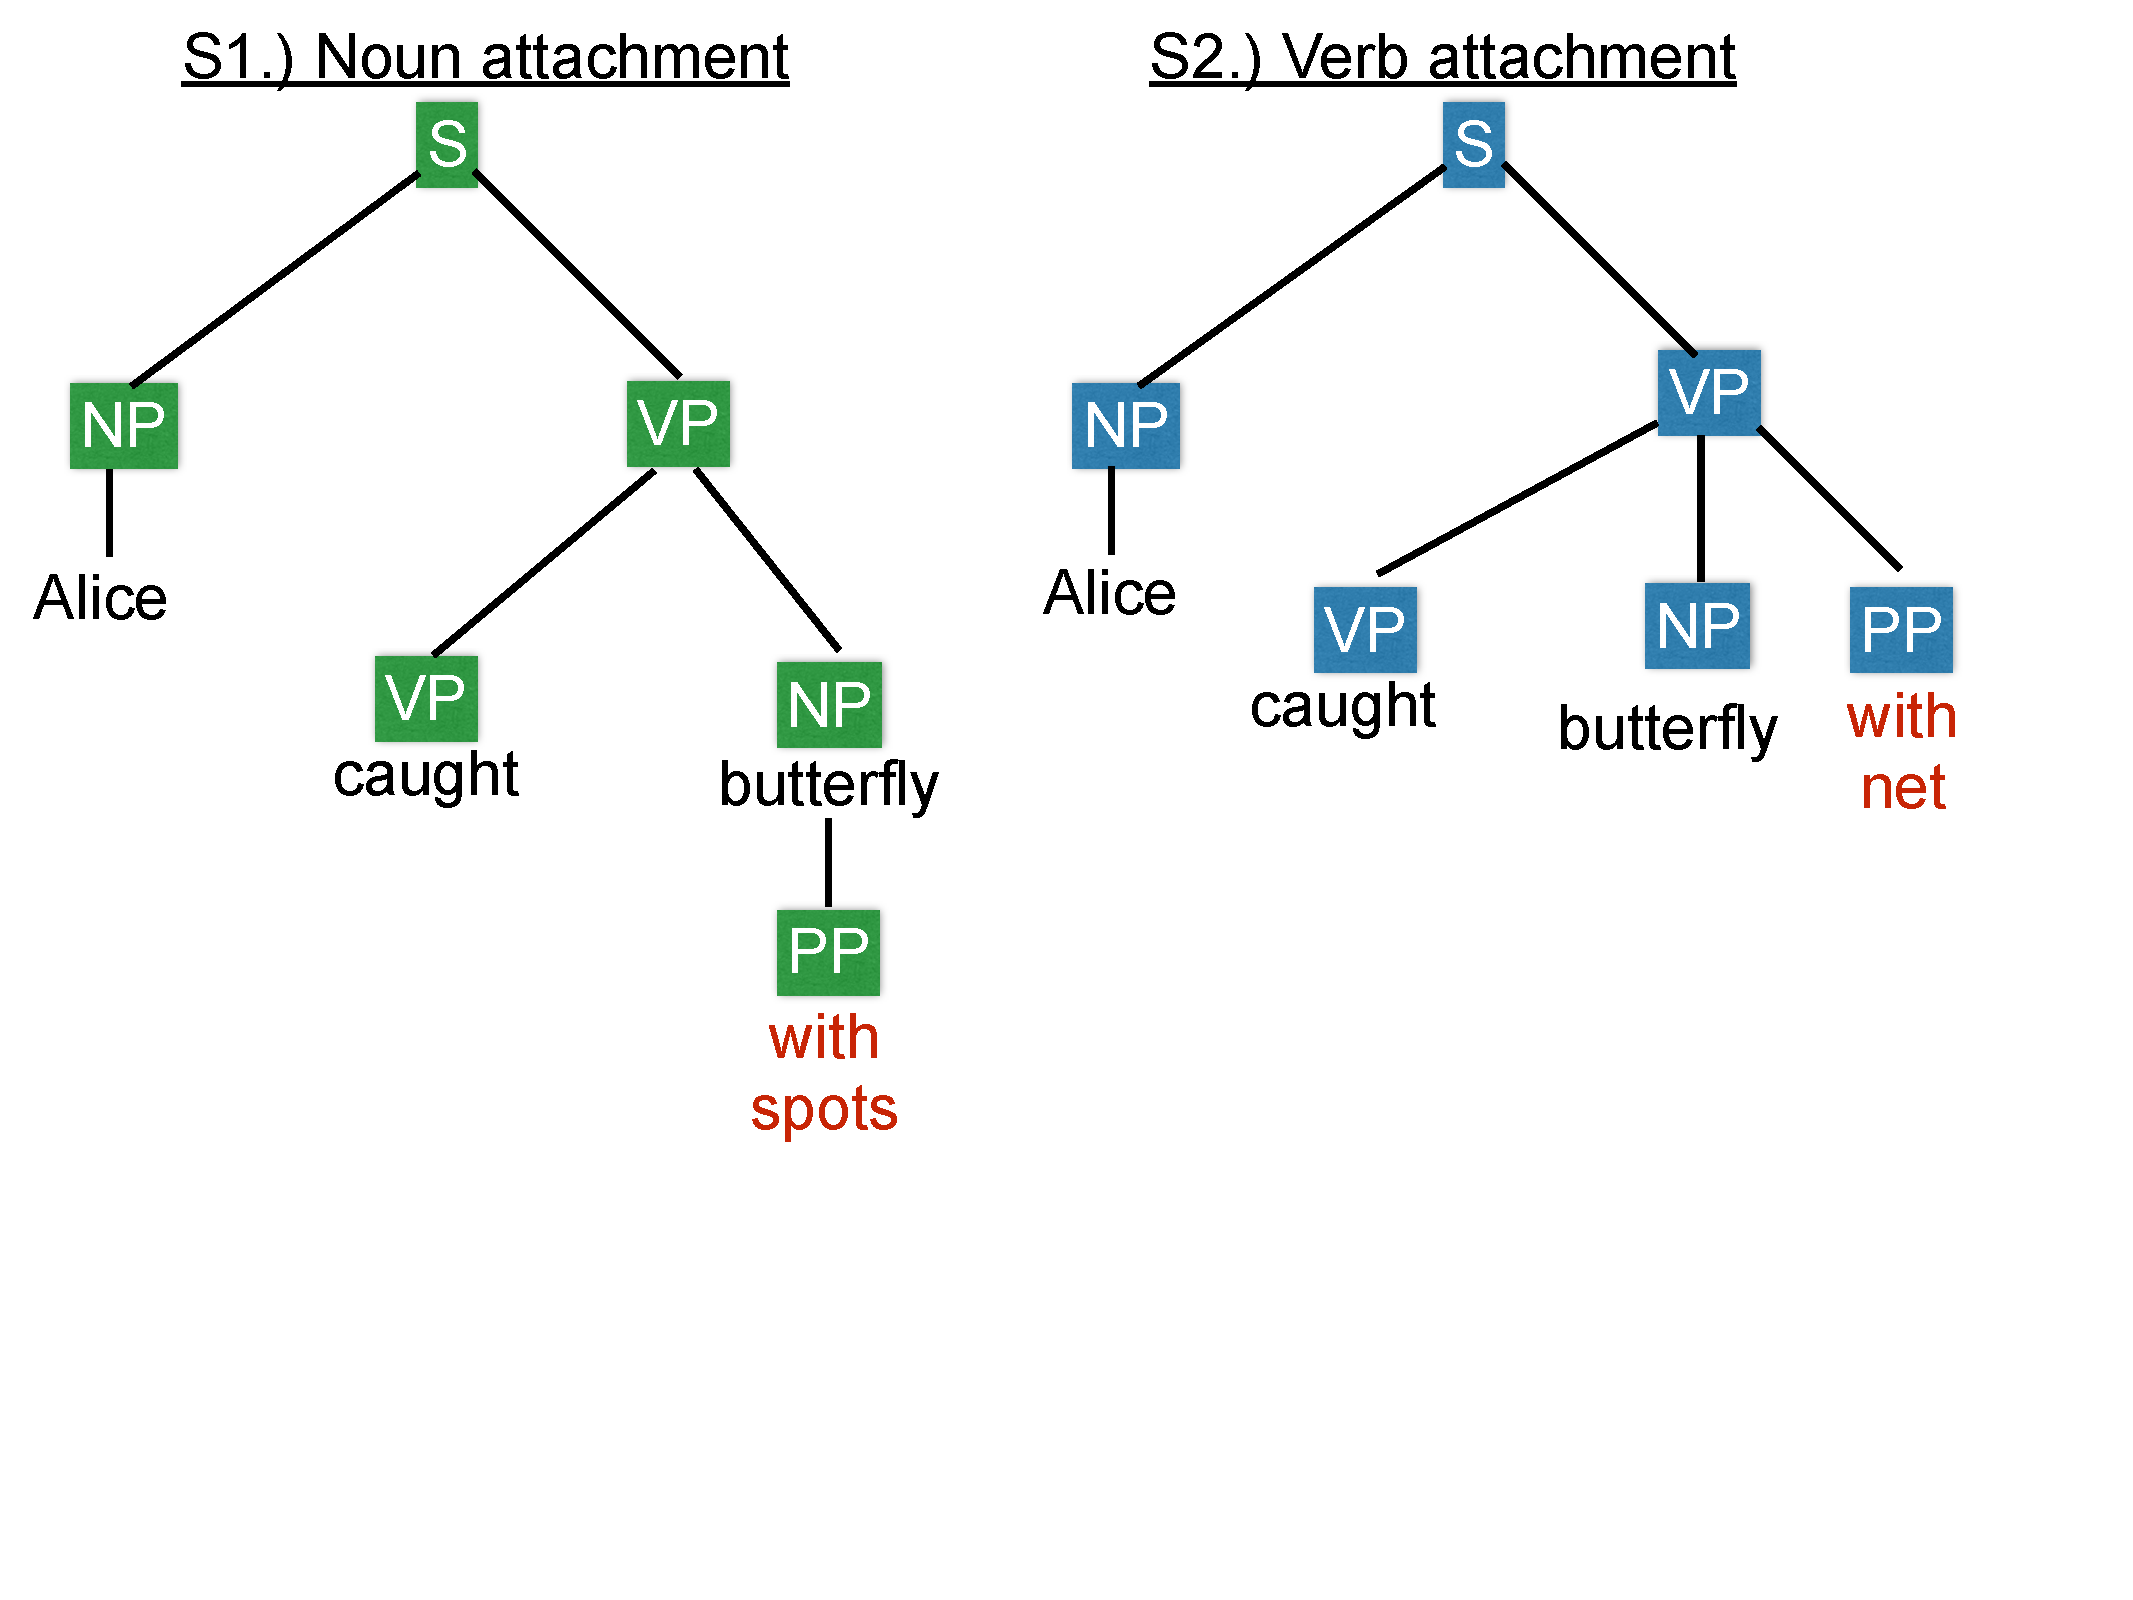
\includegraphics[width=1\columnwidth] {trees2.pdf}
\vspace*{-2.6cm}
\caption{Parse trees where the prepositional phrase (PP) attaches to the noun, and to the verb.}
%The only difference in the parse trees are the PP attachment sites, resulting in trees of different structures.}
%and hence the sentence structures are different. } 

\label{fig:deptrees}

\end{figure}



 As an example, consider the following sentences: \textit{ S1.) Alice caught the butterfly with the spots. S2.) Alice caught the butterfly with the net. }  S1 and S2 are syntactically different, this is evident from their corresponding parse trees in Figure \ref{fig:deptrees}. Specifically,  S1 and S2  differ in where their PPs attach. In  S1,  the butterfly has spots and therefore  the PP, ``with the spots'', attaches to the \textit{noun}. For relation extraction, we  obtain a \textit{binary} relation of the form:  
 $\langle$Alice$\rangle$  caught $\langle$butterfly with  spots$\rangle$.
However, in S2, the net is the instrument used for catching and therefore  the PP,  ``with the net", attaches to the \textit{verb}.  For relation extraction, we get a \textit{ternary} extraction of the form:
%\begin{itemize}
%\item[]
 $\langle$Alice$\rangle$  caught $\langle$butterfly$\rangle$ with $\langle$net$\rangle$.
%\item[] $\langle$The government$\rangle$  discovered $\langle$irregularities$\rangle$ in $\langle$June$\rangle$
%\end{itemize
 
The PP attachment problem is often defined as follows: given a PP occurring within a  sentence where there are multiple possible attachment sites for the PP, choose the most plausible attachment site. 
%Notice that in the examples we have given so far, there were only two possible attachment sites, the noun and the verb.
% as shown in Figure \ref{fig:deptrees} with a parse tree corresponding to each type.
 In the literature,  prior work going as far back as \cite{BrillR94,Ratnaparkhi1994,Collins95} has  focused on the  language pattern that causes most PP ambiguities, which is the  4-word sequence: $\{v, n1, p, n2\}$ (e.g., $\{${\em caught, butterfly, with, spots}$\}$). The task is  to   determine if  the prepositional phrase $(p,n2)$  attaches to  the verb $v$ or to the first noun $n1$.
Following common practice,  we focus on  PPs occurring as $\{v,n1,p,n2\}$ quadruples ---  we shall refer to these as  \textit{PP quads}. 

The approach we present here differs from prior work in two main ways. First, we make extensive use of semantic knowledge about nouns, verbs, prepositions, pairs of nouns, and  the discourse context in which a PP quad occurs. Table \ref{tab:knowledge}  summarizes the types of  knowledge we considered in our work. Second, in training our model, we rely on both labeled and unlabeled data, employing an expectation maximization (EM) algorithm \cite{Dempster77maximumlikelihood}. 


\begin{table}[h]
\centering
\small{
   \begin{tabular}{|p{1.8cm}|p{4.9cm}|}
     % \hline
   %&  {\bf Definition \& Example(s)}  \\
     \hline
    % \newline -receive(agent, patient, source) \\
     % \newline -isA(tea,beverage)\\
     Relations &  Noun-Noun binary relations  \newline \textit{ (Paris, located in, France)} \newline \textit{(net, caught, butterfly)}\\
     \hline
     Nouns &  Noun semantic categories \newline \textit{(butterfly, isA, animal)}  \\
     \hline
     Verbs & Verb roles \newline  \textit{caught(agent, patient, instrument)} \\
     \hline
     % \newline -(fork, used for, eating) \\
     Prepositions& Preposition  definitions \newline  
     \textit{ f(for)= used for, has purpose, ...}  
     \newline \textit{f(with)= has, contains, ...}  \\
     \hline
     Discourse &  Context \newline  $n0 \in \{n0, v, n1, p, n2\}$\\
     \hline
   \end{tabular}
   \caption{Types of background   
   knowledge used in this paper to determine PP attachment.}
     \label{tab:knowledge}
     }      
   \end{table}   
   

\begin{figure}[t]
%
\centering
%
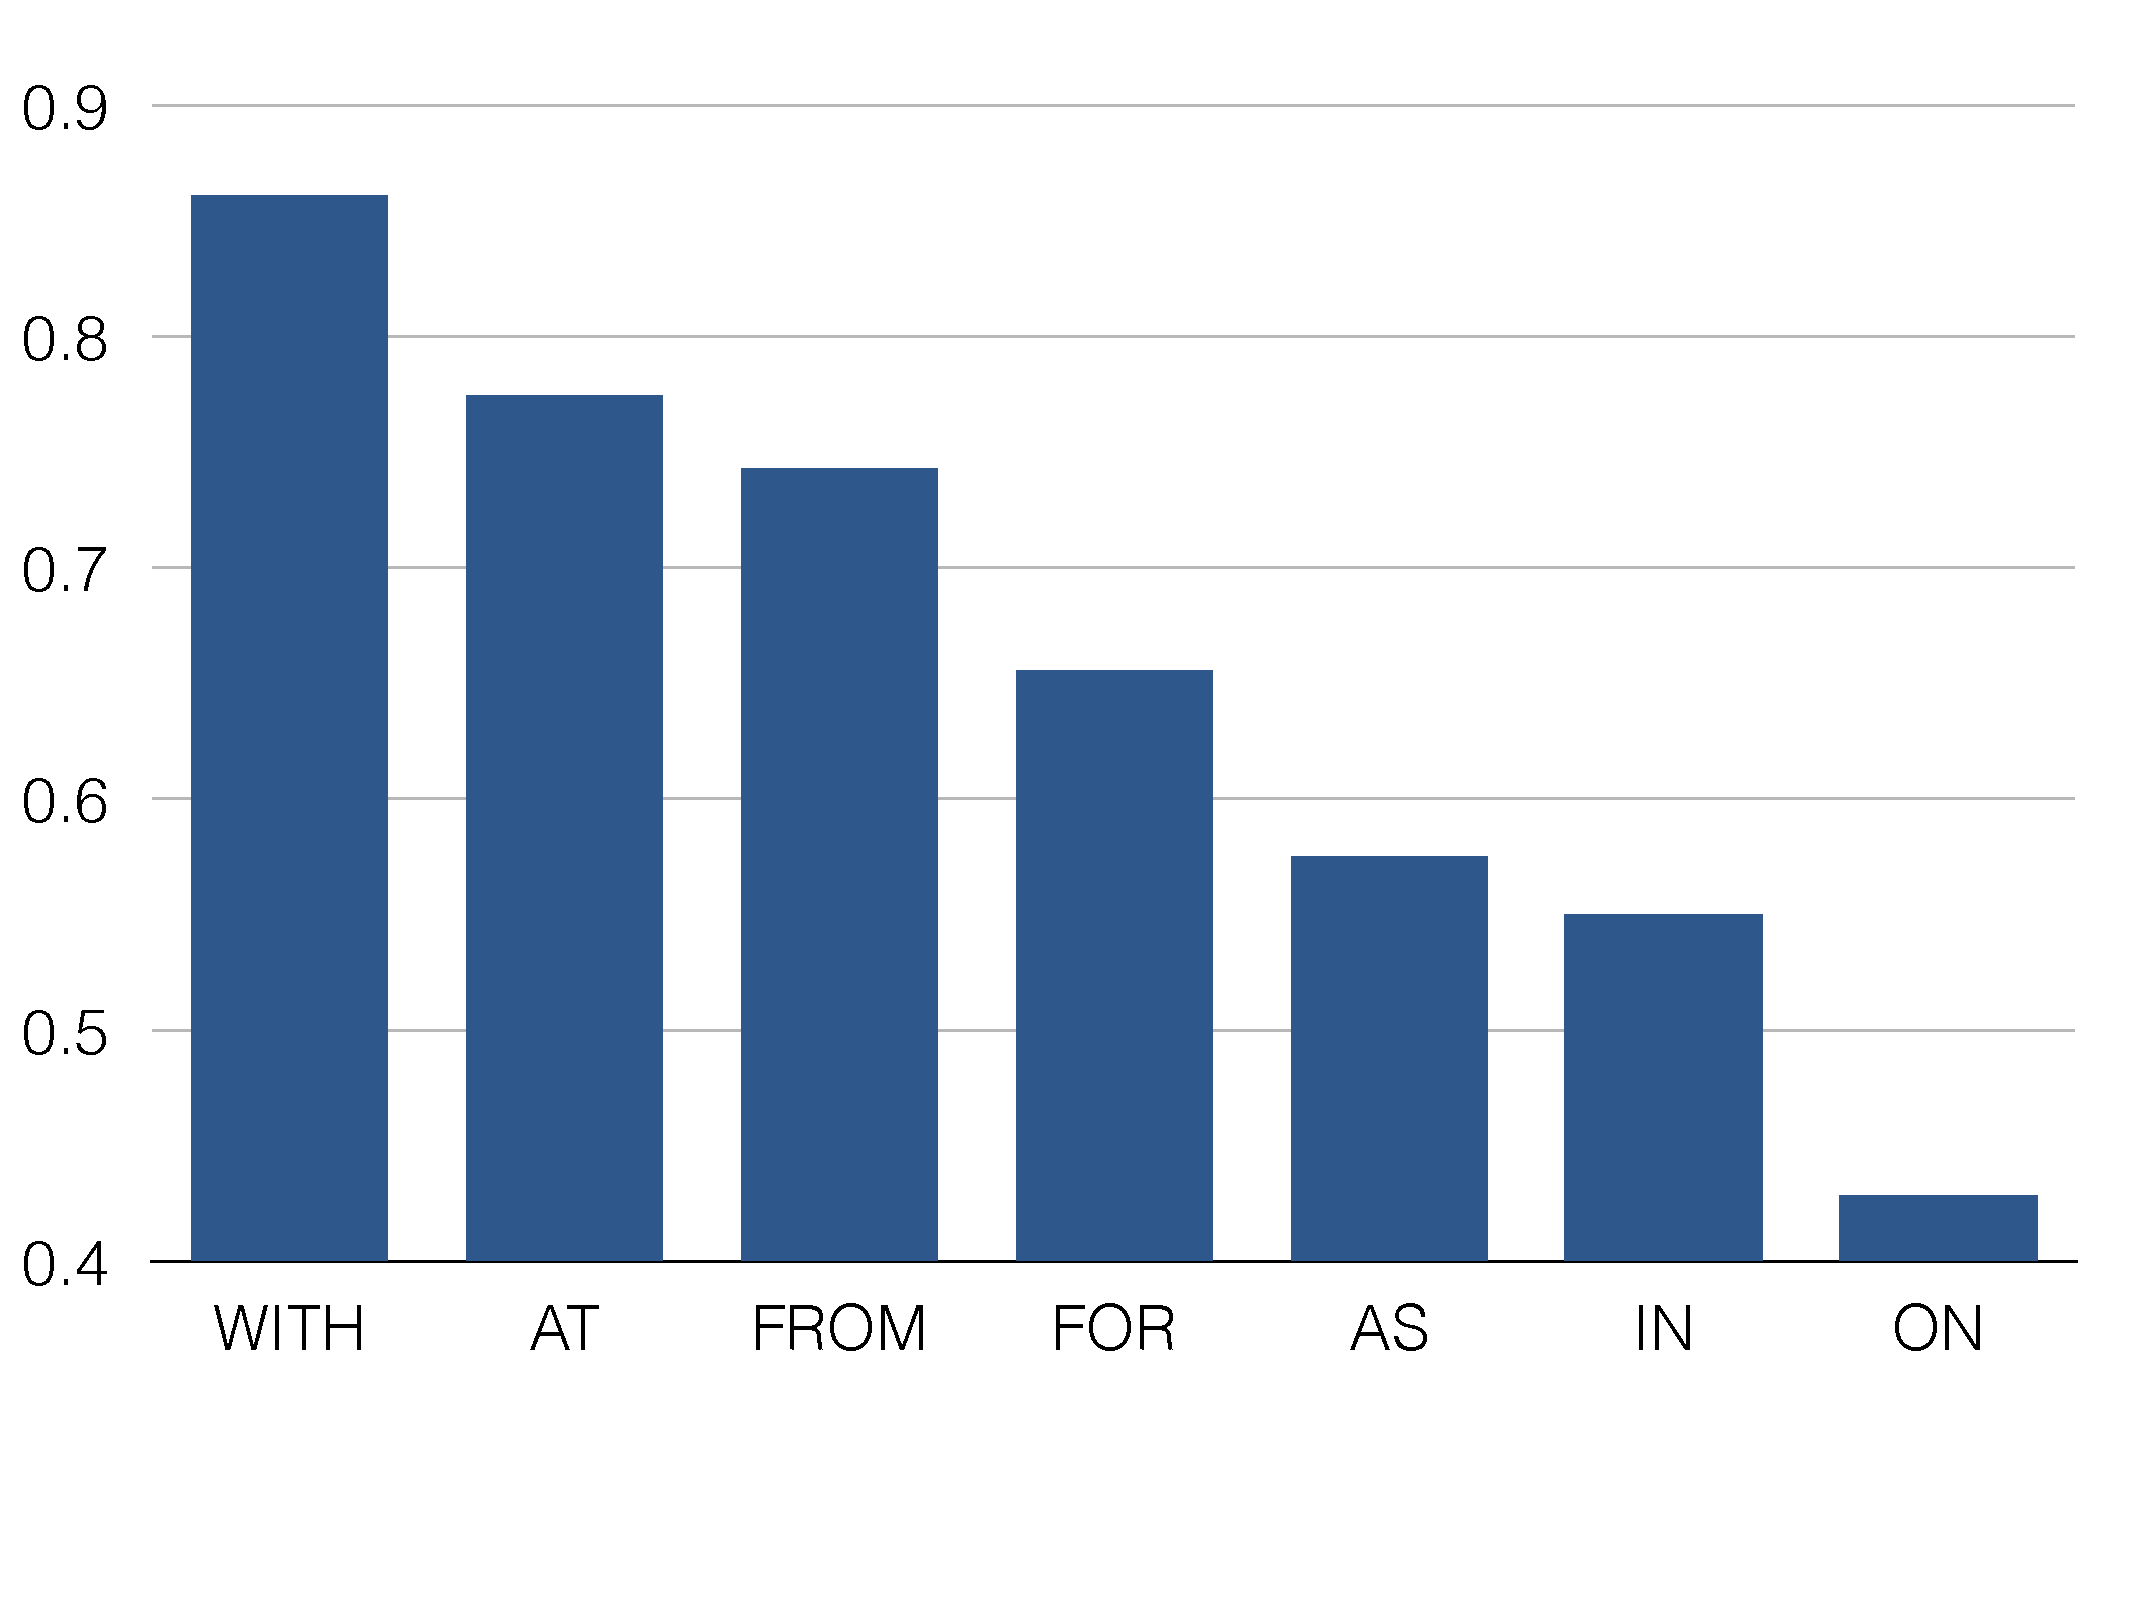
\includegraphics[width=0.80\columnwidth] {mainresults-0.pdf}
\vspace*{-0.8cm}
\caption{Dependency parser PP attachment accuracy for various frequent prepositions.}
% The only difference in the parse trees are the PP attachment sites, resulting in trees of different structures.}
% and hence the sentence structures are different. } 
%
\label{fig:parser}
%
\end{figure}  

                

\subsection{State  of  the Art}
    

\begin{figure}[t]
 %
 \centering
 %
 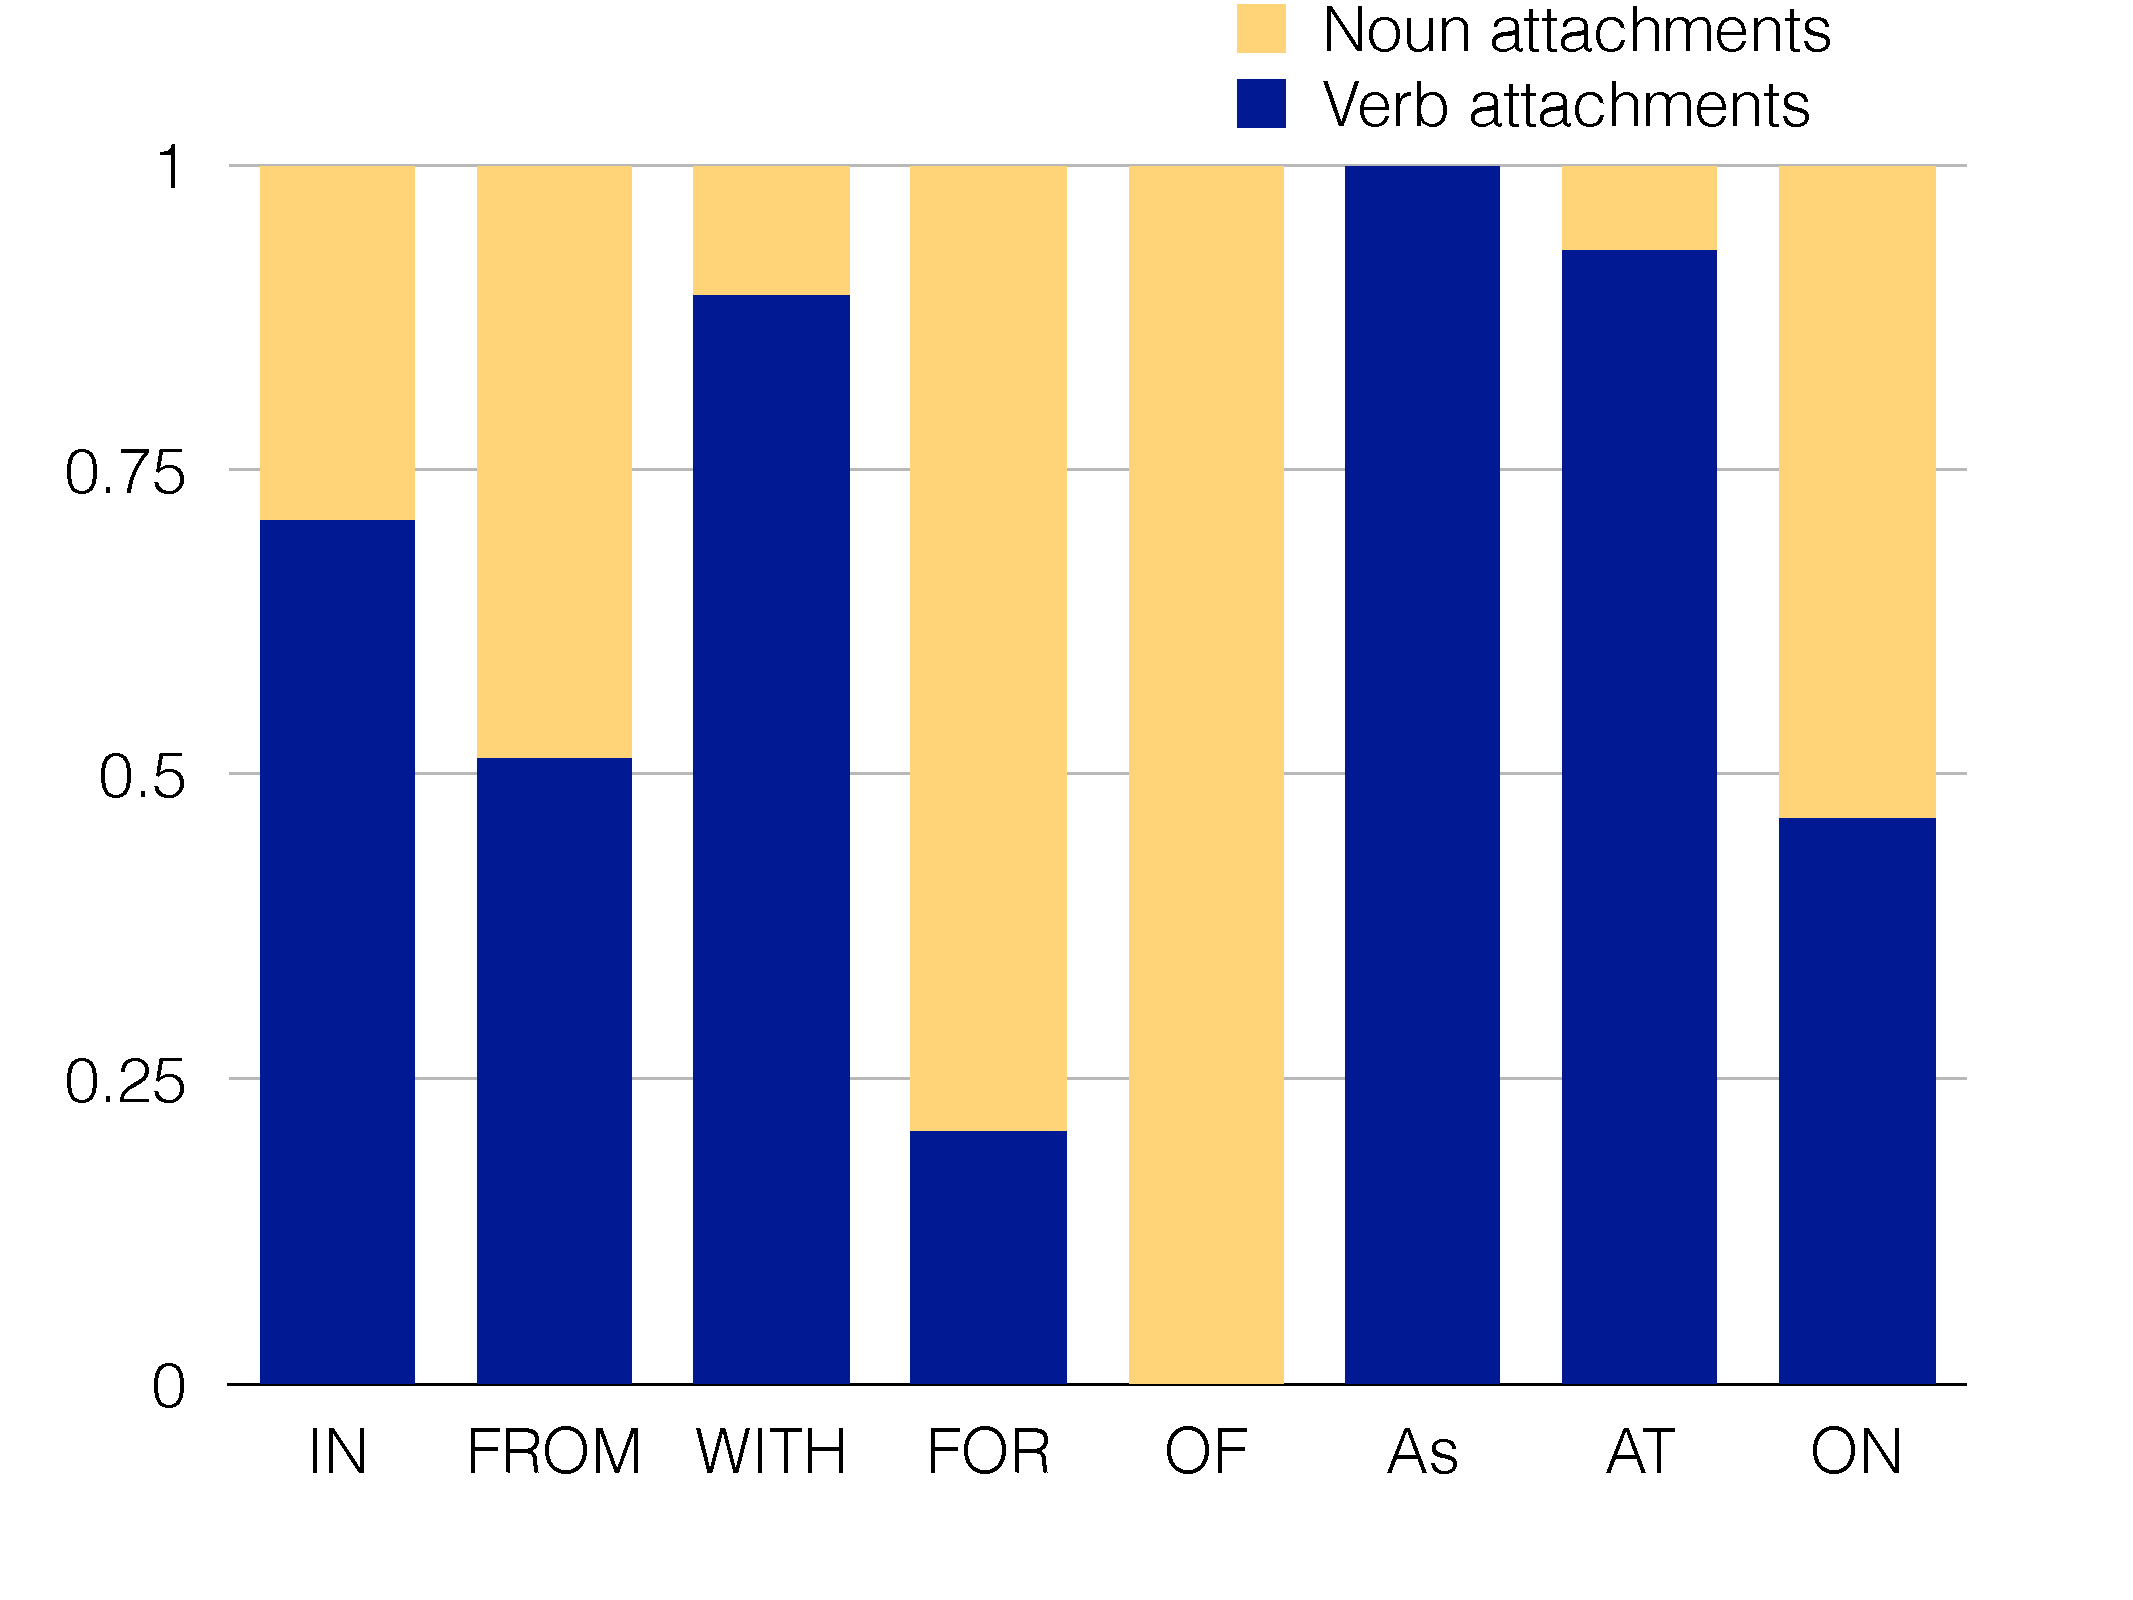
\includegraphics[width=0.85\columnwidth] {mainresults-5.pdf}
 \vspace*{-0.5cm}
 \caption{Noun vs. verb attachment proportions for frequent prepositions in the labeled NYTC dataset.}
 % The only difference in the parse trees are the PP attachment sites, resulting in trees of different structures.}
 % and hence the sentence structures are different. } 
 %
 \label{fig:distribution}
 %
 \end{figure}  

 To quantitatively assess existing tools, we analyzed performance of the widely used  Stanford parser\footnote {http://nlp.stanford.edu:8080/parser/} as of 2014,  and the established  baseline algorithm \cite{Collins95}, which has stood the test of time.
We first manually labeled PP quads from the NYTC dataset, then prepended the noun phrase appearing before the quad, effectively creating sentences made up of 5 lexical items 
$(n0\  v\  n1\  p\  n2)$.  We then applied the Stanford parser, obtaining the results summarized in Figure~\ref{fig:parser}.  The parser performs well on some prepositions, for example,  ``of", which tends to occur with noun attaching PPs as can be seen in Figure \ref{fig:distribution}.  However, for  prepositions  with an even distribution over verb and noun attachments, such as ``on", precision is as low as ~50\%. %indicating there is room for improvement.
The Collins baseline achieves 84\% accuracy on the benchmark Wall Street Journal PP dataset.  
 However, drawing a distinction in the precision of  different prepositions provides useful insights on its performance.  We re-implemented this baseline  and found that when we remove the trivial preposition,  ``of",  whose PPs are by default attached to the noun by this baseline, precision drops to 78\%. 
 This  analysis  suggests there is substantial room for improvement.
 % \highlight{For higher resolving prepositions.}


\subsection{Related Work}
\paragraph{Statistics-based Methods}
%common types of PP attachment methods in literature. 
Prominent  prior methods learn to perform PP attachment based on corpus co-occurrence statistics,  gathered either from  manually annotated training data \cite{Collins95,BrillR94} or from  automatically acquired  training data that may be noisy \cite{Ratnaparkhi98,PantelL00}.  These models collect statistics on how often a given quadruple, $\{v,n1,p,n2\}$, occurs in the training data as a verb attachment as opposed to a noun attachment.  The issue with this approach is sparsity, that is, many quadruples occuring in the test data might not have been seen in the training data.
Smoothing techniques are often employed to overcome sparsity.  For example, \cite{Collins95} proposed a back-off model that uses  subsets of the words in the quadruple, by also keeping  frequency counts of triples, pairs and single words. 
% when the test quadruple itself was not seen in the training data. 
Another approach to overcoming sparsity has been to use WordNet \cite{fellbaum98wordnet} classes, by replacing nouns with their WordNet classes \cite{Stetina97,ToutanovaMN04} to obtain less sparse corpus statistics.  Corpus-derived clusters of similar  nouns and verbs have also been used  \cite{PantelL00}.

Hindle and Rooth  proposed a lexical association approach based on how words are associated with each other \cite{HindleR93}. Lexical preference is used by  computing co-occurrence
frequencies (lexical associations) of verbs and nouns,  with prepositions. In this manner, they would discover that, for example,  the verb ``send" is highly associated with the preposition \textit{from},  indicating that in this case, the PP  is likely to be a verb attachment. 


\paragraph{Structure-based Methods}
These methods are based on  high-level  observations that are then generalized into heuristics for 
 PP attachment decisions. \cite{Kimball73}  proposed a right association method, whose premise is that a word tends to attach to another word immediately to its right.
\cite{Frazier78} introduced a minimal attachment method, which posits that  words attach to an existing non-terminal word using the fewest additional syntactic nodes. 
While simple, in practice these methods have been found to perform poorly \cite{WhittemoreFB90}.

\paragraph{Rule-based Methods}
%Different from frequency counting,
\cite{BrillR94}  proposed methods that
 learn  a set of transformation rules from a corpus. 
 %The  rules are then applied to a given PP attachment instance.
 %  and therefore, unlike the statistical methods, it is
%not necessary to store   tables  word dependencies or co-occurrence probabilities.
The rules can be too  specific to have broad applicability, resulting in low recall. 
To address low recall, knowledge about nouns, as found in  WordNet,   is used to replace certain
words in rules with  their WordNet classes. 
%This allows rules to match more  PP attachment instances


\paragraph{Parser Correction Methods}
The  quadruples formulation of the PP problem  can be seen as a simplified setting. This is because, with quadruples,  there is no need to deal with complex sentences but only well-defined quadruples of the form $\{v,n1,p,n2\}$. Thus in the quadruples setting, there are only two possible attachment sites for the PP, the $v$ and $n1$.  An alternative setting is to  work in the context of full sentences. In this setting the problem is cast as a dependency parser correction problem \cite{AttererS07,Agirre08,AnguianoC11}. That is, given a dependency parse of a sentence, with potentially incorrect PP attachments, rectify it such that the prepositional phrases attach to the correct sites. Unlike our approach, these methods do not take semantic knowledge into account.

\paragraph{Sense Disambiguation}
In addition to prior work on prepositional phrase attachment, a highly related problem is preposition sense disambiguation \cite{Hovy2011,SrikumarR13}.  Even a
syntactically correctly attached PP can  still  be semantically ambiguous with respect to questions of machine reading such as \textit{where, when,} and \textit{why}. 
Therefore, when extracting information from prepositions, the problem of preposition sense disambiguation (semantics) has to be addressed in addition to prepositional phrase attachment disambiguation (syntax). In this paper, our focus is on the latter. 

\begin{table*}[th]
%
\centering
%
\begin{tabular}{ |l| l|l|l| }
\hline
{\bf Feature Type} & {\bf \#} &  {\bf Feature}  & {\bf Example}\\
\hline

Noun-Noun Binary Relations &  & \textbf{Source: SVOs} & \\ 
   & F1. &  $svo(n2,v,n1)$  &  For q1; $(net,caught,butterfly)$\\ 
 % & $svo(t2,v,t1)$  &  For q1; $svo(< device>,caught, <animal>)$\\ 
& F2. &  $\forall i : \exists sv_{i}o; $  $svo(n1,v_i,n2)$ & For q2; $(butterfly,has,spots)$ \\ 
%& & & For q2; $(butterfly,can $ $have,spots)$\\ 
& & & For q2; $(butterfly, can $ $see,spots)$\\ 

   Noun  Semantic Categories  &  &  {\bf Source: $\mathcal{T}$ }  & \\
                & F3. &  $\forall t_i \in \mathcal{T};$ $isA(n1,t_i)$ & For q1 $isA(butterlfy,animal)$\\ 
                   & F4. &  $\forall t_i \in \mathcal{T};$  $isA(n2,t_i)$ & For q2 $isA(net,device)$\\ 
                                                                                                          
  Verb  Role Fillers & & \textbf{Source: VerbNet} & \\ 
  & F5. &   $hasRole(n2, r_{i})$ &  For q1; $(net, instrument)$ \\
%   &  &  &   For q3; $(child, beneficiary)$ \\   

Preposition Relational  &  &  \textbf{Source: $\mathcal{M}$} & \\ 
  Definitions & F6. & $def(prep,v_i)$ $\forall i :$ &  
\\ 
         &  & $\exists sv_{i}o; v_i \in  \mathcal{M}$ $ \wedge$  &  
       \\ 
          &  &  $svo(n1,v_i,n2)$  &  For q2;
                    $def(with,has)$ \\ 
 % &  &  $svo(n1,v_i,n2)$  & For q2; $(butterfly,can $ $have,spots)$\\  
 
 Discourse Features &  & \textbf{Source: Sentence(s), $\mathcal{T}$} & \\ 
             & F7. &  $\forall t_i \in \mathcal{T}; isA(n0,t_i)$ &  $n0 \in \{n0, v, n1, p, n2\}$ \\
             %$isA(n0,t_i)$ & For  $n0 \in \{n0, v, n1, p, n2\}$ \\

Lexical  Features& &  {\bf Source: PP quads} & For q1;\\ 
& F8.  & $(v, n1, p, n2)$ & $(caught,butterfly,with,net)$ \\
& F9. & $(v, n1, p)$ & $(caught,butterfly,with)$ \\
& F10. & $(v, p, n2)$ & $(caught,with,net)$ \\ 
& F11. & $(n1, p, n2)$ &$(butterfly,with,net)$ \\ 
& F12.  & $(v,p) $ & $(caught,with)$\\ 
& F13.  & $(n1,p) $ & $(butterfly,with)$\\ 
& F14. & $(p,n2) $ & $(with,net)$ \\ 
   &F15.  &$(p) $ & $(with)$\\  
\hline
\end{tabular}
\caption{Types of  features considered in our experiments. All features have values of 1 or 0.  The PP quads used as running examples are:  $q1=\{caught, butterfly, with, net\}: V$, $q2=\{caught, butterfly, with, spots\}: N$.}
\label{tab:featurevectors}
\end{table*}
   
 

\subsection{Methodology} 
%\highlight{Do not refer to features but rather to feature types.}
%Attributes, Ownership/Possession
%[NP’s NP]: Mary’s laptop or car’s wheel  but also Mary’s brother or  France’s political elite, government 's explanation,  Netanyahu 's frosty visit 
%[NP of NP]:  eyes of the baby, economy of Asia,  but also fact of life, a lot of chances 
%[NP has/have NP]:  Bob has brown eyes, Bob has a cat, cats have fur, cake has nuts, 
%[NP is made of NP]: foil made of aluminum 
%[NP contains/consists of NP]:  wine contains alcohol, water consists of hydrogen



Our approach consists of first generating features from background knowledge and then training a model to learn with these features.
%extracted from both labeled and unlabeled data. 
 The types of features considered in our experiments are  summarized  in Table~\ref{tab:featurevectors}.  The choice of features was motivated by our empirically driven characterization of the problem as follows:
\begin{table}[h]
\centering
\begin{tabular}{p{7cm}}
\textit{(Verb attach) $\longrightarrow$ v $\langle$has-slot-filler$\rangle$ n2} \\
\hline
\textit{(Noun attach a.) $\longrightarrow$ n1 $\langle$described-by$\rangle$ n2}\\
\textit{(Noun attach b.) $\longrightarrow$ n2 $\langle$described-by$\rangle$ n1}\\
\end{tabular}
\label{tbl:example}
\end{table}

That is, we found that for verb-attaching PPs, $n2$  is usually a role filler for the verb, e.g., the net fills the role of an instrument for the verb $catch$. On the other hand,  for noun-attaching PPs,  one noun describes or elaborates on the other. In particular, we found  two kinds of noun attachments. For the first kind of noun attachment,  the second noun $n2$ describes  the first noun $n1$, for example $n2$ might be  an attribute or property of $n1$, as in   the spots($n2$) are an attribute of the butterfly ($n1$).  And for the second kind of noun attachment, the first noun $n1$ describes the second noun $n2$, as  in the PP quad $\{${\em expect, decline, in, rates}$\}$,  where the PP ``in rates'', attaches to the $noun$. The decline:$n1$ that is expected:$v$ is in the rates:$n2$. We sampled $50$ PP quads from the WSJ dataset and found that every labeling could be explained using our characterization.  
 We make this labeling available with the rest of the datasets.



We next describe in more detail how each type of feature is derived from the  background knowledge  in Table~\ref{tab:knowledge}.

We generate boolean-valued features for all the feature types we describe in this section.

\subsubsection{Noun-Noun Binary Relations}
%This type of knowledge refers to binary relations between pairs of nouns. 
The noun-noun  binary relation features, F1-2 in Table \ref{tab:featurevectors}, are boolean features   $svo(n1,v_i,n2)$ (where $v_i$ is any verb) and $svo(n2,v,n1)$ (where $v$ is the verb in the PP quad, and the roles of $n2$ and $n1$ are reversed). These features describe diverse semantic relations between pairs of nouns (e.g.,   \textit{butterfly-has-spots},   \textit{clapton-played-guitar}).  To obtain this type of knowledge, we dependency parsed all sentences in the 500 million English web pages of the ClueWeb09 corpus, then extracted subject-verb-object (SVO) triples from these parses, along with the frequency of each SVO triple in the corpus.  The value of any given feature $svo(n1,v_i,n2)$ is defined to be 1 if that SVO triple was found at least $3$ times in these SVO triples, and 0 otherwise.


To see why these relations are relevant, let us suppose that  we have  the knowledge that \textit{butterfly-has-spots}, $svo(n1,v_i,n2)$. From this, we can  infer that the PP in $\{caught,butterfly, with, spots\}$ is likely to attach to the noun.   Similarly,  suppose we  know that \textit{net-caught-butterfly}, $svo(n2,v,n1)$. The fact   that a net can be used to catch a butterfly can be used to predict that  the  PP in\\ $\{caught,butterfly, with, net\}$ is likely to attach to the verb.   

\subsubsection{Noun Semantic Categories} 

Noun semantic type features, F3-4, are boolean features   $isA(n1,t_i)$ and $isA(n2,t_i)$ where $t_i$ is a noun category in a noun categorization  scheme   $\mathcal{T}$ such as WordNet classes. 
Knowledge about semantic types of nouns, for example  that a butterfly is an animal, enables extrapolating predictions to other PP quads that contain nouns of the same type. % For example,  $\{caught,<$$animal$$>, with, spots\}$. 
We ran experiments with several noun categorizations including WordNet classes,  knowledge base ontological types,  and an unsupervised noun categorization produced by clustering  nouns based on the verbs and adjectives with which they co-occur  (distributional similarity).  

\subsubsection{Verb Role Fillers} 
The verb role feature, F5, is a boolean feature $hasRole(n2, r_{i})$ where $r_i$ is a role that  $n2$ can fulfill for the verb  $v$ in the PP quad, according to background knowledge. Notice that  if  $n2$ fills a role for the verb, then the PP is a verb attachment.  Consider the quad $\{caught,butterfly, with, net\}$, if we know that  a net can play the role of an \textit{instrument} for the verb \textit{catch}, this suggests a likely verb attachment.  We obtained background knowledge of verbs and their possible roles  from the VerbNet lexical resource ~\cite{KipperKRP08}. 
From VerbNet we obtained $2,573$ labeled  sentences containing PP quads (verbs in the same VerbNet group are considered synonymous), and the  labeled semantic roles  filled by the second noun $n2$ in the PP quad.  We use these example sentences  to label similar  PP quads, where similarity of PP quads is defined by  verbs from the same VerbNet group. 

%See feature 5 in Table~\ref{tab:featurevectors}.

\subsubsection{Preposition  Definitions}
The preposition  definition feature, $F6$, is a boolean feature $def(prep,v_i)=1$ $if$ $\exists v_i \in  \mathcal{M}$ $ \wedge$  $svo(n1,v_i,n2)=1$, where $ \mathcal{M}$ is a definition mapping of prepositions to verb phrases.   This mapping defines prepositions, using verbs in our ClueWeb09 derived SVO corpus, in order to capture their senses using verbs; it contains definitions such as \textit{def(with, *) = contains, accompanied by, ... }.   If  ``with" is  used in the  sense of ``contains" , then the PP  is a likely noun attachment, as in $n1$ contains $n2$ in the quad $ate, cookies, with, cranberries$. However, if  ``with" is  used in the sense of  ``accompanied by", then the PP is a likely verb attachment, as in the quad $visted, Paris, with, Sue$.

% when used in conjunction with  binary relation features.
To obtain the mapping, we took the labeled PP quads (WSJ, \cite{Ratnaparkhi1994}) and computed a ranked list of verbs from SVOs, that appear frequently between  pairs of nouns  for a given preposition.
 %, for a given attachment site verb(v) or noun(n). 
 % We obtained a large collection of such mappings.
 Other   sample mappings are:  \textit{def(for,*)= used for},   \textit{def(in,*)= located in}. Notice that this feature $F6$ is a selective, more targeted version of $F2$.
 %\textit{f(from,n)= comes from, born in, ...}.




\subsubsection{Discourse and Lexical Features}
The  discourse feature, $F7$,  is  a boolean feature  $isA(n0,t_i)$, for each noun category $t_i$ found in a noun category ontology  $\mathcal{T}$  such as WordNet semantic types. 
The context of the PP quad can contain relevant information  for  attachment decisions. We  take into account the noun preceding  a PP quad, in particular, its semantic type. This in effect makes the PP quad into a  PP 5-tuple:  $\{n0, v, n1, p, n2\}$, where the $n0$  provides additional context.
% See feature $7$ in Table~\ref{tab:featurevectors}.

%\subsection{}
%\subsubsection{ Features}
Finally, we  use  lexical features in the form of PP quads, features F8-15.  To overcome sparsity of  occurrences of PP quads, we also use counts of shorter sub-sequences, including  triples, pairs and singles. We only use sub-sequences that contain the preposition, as the preposition has been found to be highly crucial in PP attachment decisions \cite{Collins95}.
% See features $8-15$ in Table~\ref{tab:featurevectors}.
   
\subsection{Disambiguation Algorithm}
We use the described features to train a  model for  making PP attachment decisions.
Our goal is to compute $\mathbb{P}(y|x)$,   the probability that the PP $ (p,n2)$ in the tuple $\{v,n1,p,n2\}$ attaches to the  \textit{verb (v)} , $y=1$ or  to the $noun (n1)$, $y=0$, given a feature vector $x$ describing that tuple.
As input to training the model, we are given a collection of PP quads, $D$ where  $d_i \in \mathcal{D}: d_i=\{v,n1,p,n2\} $. A small subset,
$D^l \subset \mathcal{D}$   is labeled data, thus for each $d_i \in D^l$ we know the corresponding $y_i$. The  rest of the quads, $D^u$,  are unlabeled, hence their corresponding $y_i$s are unknown.
%In short, we have a  disjoint partitioning such that $\mathcal{D} = D^l \cup D^u $, where $|D| =N$  or equivalently,   $|D^l \cup D^u| = N$, and $|D^l| << |D^u|$.
From each PP quad $d_i$, we extract a feature vector $x_i$ according to the feature generation process  discussed earlier.. 
%Thus we have  feature vectors $\mathcal{X} =\{ x_1, .., x_N\}$.

\subsubsection{Model}
To  model $\mathbb{P}(y|x)$, there a various possibilities. One could use a generative model (e.g., Naive Bayes) or a discriminative model ( e.g., logistic regression). In our experiments we used both kinds of models, but found the discriminative model performed better. Therefore, we present details only for our discriminative model.  We use the  logistic function: 
%$\mathbb{P}(y|x, \vec \theta)  =  \frac{e^{\vec \theta x}}{1+ e^{\vec \theta x}}$,
 \begin{equation*}
 \mathbb{P}(y|x, \vec \theta)  =  \frac{e^{\vec \theta x}}{1+ e^{\vec \theta x}}
\end{equation*}
 where $\vec \theta$  is a vector of model parameters. To estimate these parameters,  we could use the labeled data as training data and  use standard   gradient descent  to minimize the logistic regression cost function. However, we also leverage the unlabeled data.  

 
 \subsubsection{Parameter Estimation}
 To estimate model parameters based on both labeled and unlabeled data, we use an Expectation Maximization (EM) algorithm. 
% The EM algorithm enables parameter estimation in models with incomplete data. 
 %In our case, the data is incomplete because the $D^u$ labels are unknown. 
 EM estimates model parameters that maximize the expected log likelihood of the full (observed and unobserved) data.  

Since we are using a discriminative model, our likelihood function is  a  conditional likelihood function:
  \begin{align}\label{eqlikelihood}
  \mathcal{L}(\theta)  &=\sum_{i=1}^{N} \mbox{ln }  \mathbb{P}(y_i|x_i)  \nonumber \\
     &= \sum_{i=1}^{N}  y_i \theta^{T}x_i - \mbox{ln } (1+ exp ( \theta^{T}x_i)) 
   \end{align}
where $i$ indexes over the $N$ training examples.
  
  

The  EM algorithm produces parameter estimates that correspond to a local maximum in the expected log likelihood of the data under the posterior distribution of the labels, given by: \\   $\arg\max\limits_{\theta}  E_{p(y|x,\theta)} [ \mbox{ln } \mathbb{P}(y|x,\theta)]$.  In the E-step, we use the current parameters $\theta^{t-1}$ to compute the posterior distribution over the $y$ labels, give by $\mathbb{P}(y|x, \theta^{t-1})$.   We then use this posterior distribution to find the expectation of the log of the complete-data conditional likelihood, this expectation is given by  $\mathcal{Q}({\bf\theta, \theta^{t-1})}$, defined as:

  \begin{align}
\mathcal{Q}(\theta,  \theta^{t-1})  &=\sum_{i=1}^{N} E_{\theta^{t-1}} [ \mbox{ln } \mathbb{P}(y|x,\theta)]  
    \end{align}

In the M-step, a new estimate $\theta^t$ is then produced, by maximizing this $Q$ function with respect to $\theta$:
\begin{equation} \label{empameterupdate}
{\bf \theta^{t}} =\arg\max\limits_{\theta}\mathcal{Q}({\bf\theta, \theta^{t-1})}
\end{equation}

EM iteratively computes  parameters $\theta^0, \theta^1, ...\theta^{t}$,  using the above update rule at each iteration $t$, halting when there is no further improvement in the value of the $Q$ function.  Our algorithm is summarized in Algorithm 1.  The M-step solution for $\theta^t$ is obtained using gradient ascent to maximize the $Q$ function.  

 \begin{algorithm}
 \caption{The EM algorithm  for PP attachment}
 \label{algorithm}
 \begin{algorithmic}
 \STATE \textbf{Input:}  $\mathcal{X}, \mathcal{D} = D^{l} \cup D^{u}$\\
 %\STATE \textbf{Input:} Prior Knowledge  $\mathcal{K}$ \\
 \STATE \textbf{Output:} $\theta^{T}$
 %\STATE  $\mathcal{X} =getFeatureVectors(\mathcal{D})$
 %\STATE  $\mathcal{X} =\{ x_1, .., x_N\}$
 \FOR{t = 1 . . . T}
   \STATE \textbf{E-Step:}
   \STATE Compute $p(y|x_i, \theta^{t-1})$\\
   \STATE $x_i: d_i\in D^u$; $p(y|x_i, \vec \theta)  =  \frac{e^{\vec \theta x}}{1+ e^{\vec \theta x}}$  \\
   \STATE $x_i: d_i \in D^{l}$; $p(y|x_i)= 1$ if  $y=y_i,$ else $0$ \\
   \STATE \textbf{M-Step:} 
   \STATE Compute new parameters, $\theta^{t}$\\
   \STATE ${\bf \theta^{t}}$ $=\arg\max\limits_{\theta}\mathcal{Q}({\bf\theta, \theta^{t-1})}$
   \vspace{-0.4cm}
   \begin{multline*}
    \mathcal{Q}(\theta,  \theta^{t-1})  =\sum_{i=1}^{N}\sum_{y\in\{0,1\}}   p(y|x_i,\theta^{t-1}) \times\\( y\theta^{T}x_i - \mbox {ln}  (1+ exp ( \theta^{T}x_i)) ) 
   \end{multline*}
    		
     \IF{convergence($\mathcal{L}(\theta),  \mathcal{L}(\theta^{t-1}))$}
     	\STATE \textbf{break}\\
     \ENDIF
 \ENDFOR
 \RETURN $\theta^{T}$
 \end{algorithmic}
 \end{algorithm} 
 
 



\subsection{Experimental Evaluation}
We evaluated our method on several datasets containing PP quads of the form $\{v,n1,p,n2\}$.   The task is to predict if the  PP ($p,n2$) attaches to the verb $v$ or to the first noun $n1$. 


\subsubsection{Experimental Setup}\label{experimentalsetup}

\begin{table}[t]
%
\centering
%
\begin{tabular}{|l|l|l|}
\hline
{\bf DataSet} &  {\bf  \# Training quads} & {\bf \# Test quads} \\
\hline
\multicolumn{3}{|c|}{Labeled data} \\
    \hline
WSJ &  20,801 & 3,097 \\
NYTC & 0 & 293  \\
 WKP & 0 & 381  \\
      \hline
 \multicolumn{3}{|c|}{Unlabeled data} \\
      \hline
        %WSJ & - & - \\
         %NYTC & - & - \\
          WKP  & 100,000 & 4,473,072 \\
         
\hline
\end{tabular}
\caption{Training and test datasets used in our experiments. }
%\tom{What does "-" mean in this table?  If zero, let's use "0"}}
\label{tab:datasets}
\end{table}
     
    
     
\paragraph{Datasets}
Table~\ref{tab:datasets} shows the datasets used in our experiments. 
As labeled training data, we used the Wall Street Journal  (WSJ) dataset. For the unlabeled  training data, we extracted  PP quads from Wikipedia (WKP) and randomly selected $100,000$ which we found  to be a sufficient amount of unlabeled data.
The largest labeled test dataset is  WSJ
but it is also made up of a large fraction, of  ``of" PP quads, 30\% , which trivially attach to the noun, as already seen  in Figure \ref{fig:distribution}.
%and in general it is more comprehensive in the kind of prepositions it contains.
 The New York Times (NYTC) and Wikipedia (WKP) datasets are  smaller but contain fewer proportions  of ``of" PP quads, 15\%,  and 14\%, respectively. 
  %with a focus on  frequently used prepositions.
  Additionally, we applied our  model to over 4 million unlabeled 5-tuples from Wikipedia. We make this data available for download,  along with our manually labeled NYTC and WKP datasets.
For the WKP \& NYTC corpora,  each quad has a  preceding noun, $n0$, as context, resulting in PP 5-tuples of the form:  $\{n0,v,n1,p,n2\}$. The WSJ dataset was only available to us in the form of  PP quads with no other sentence information.

\begin{table}[t]
\centering
\begin{tabular}{|l|l|l|l|l|}
\hline
& PPAD& PPAD- &Coll-& Stan-\\
& & NB &ins& ford\\
\hline
WKP &  \bf{0.793} &	0.740&	0.727&	0.701\\
\hline
WKP  & \bf{0.759} &	0.698&	0.683&	0.652 \\
\textbackslash of  & & & & \\
\hline
NYTC & \bf{0.843}	& 0.792	&0.809	&0.679\\
\hline
NYTC& \bf{0.815}	& 0.754&	0.774&	0.621\\
\textbackslash of  & & & & \\
\hline
WSJ & \bf{0.843}&	0.816&	0.841& N\textbackslash A \\
\hline
WSJ & \bf{0.779}	& 0.741&	0.778&N\textbackslash A  \\
\textbackslash of  & & & & \\
\hline
\end{tabular}
 \caption{PPAD  vs. baselines.}
   \label{fig:resultmain}
\end{table}
    

\begin{figure}[t]
%
\centering
%
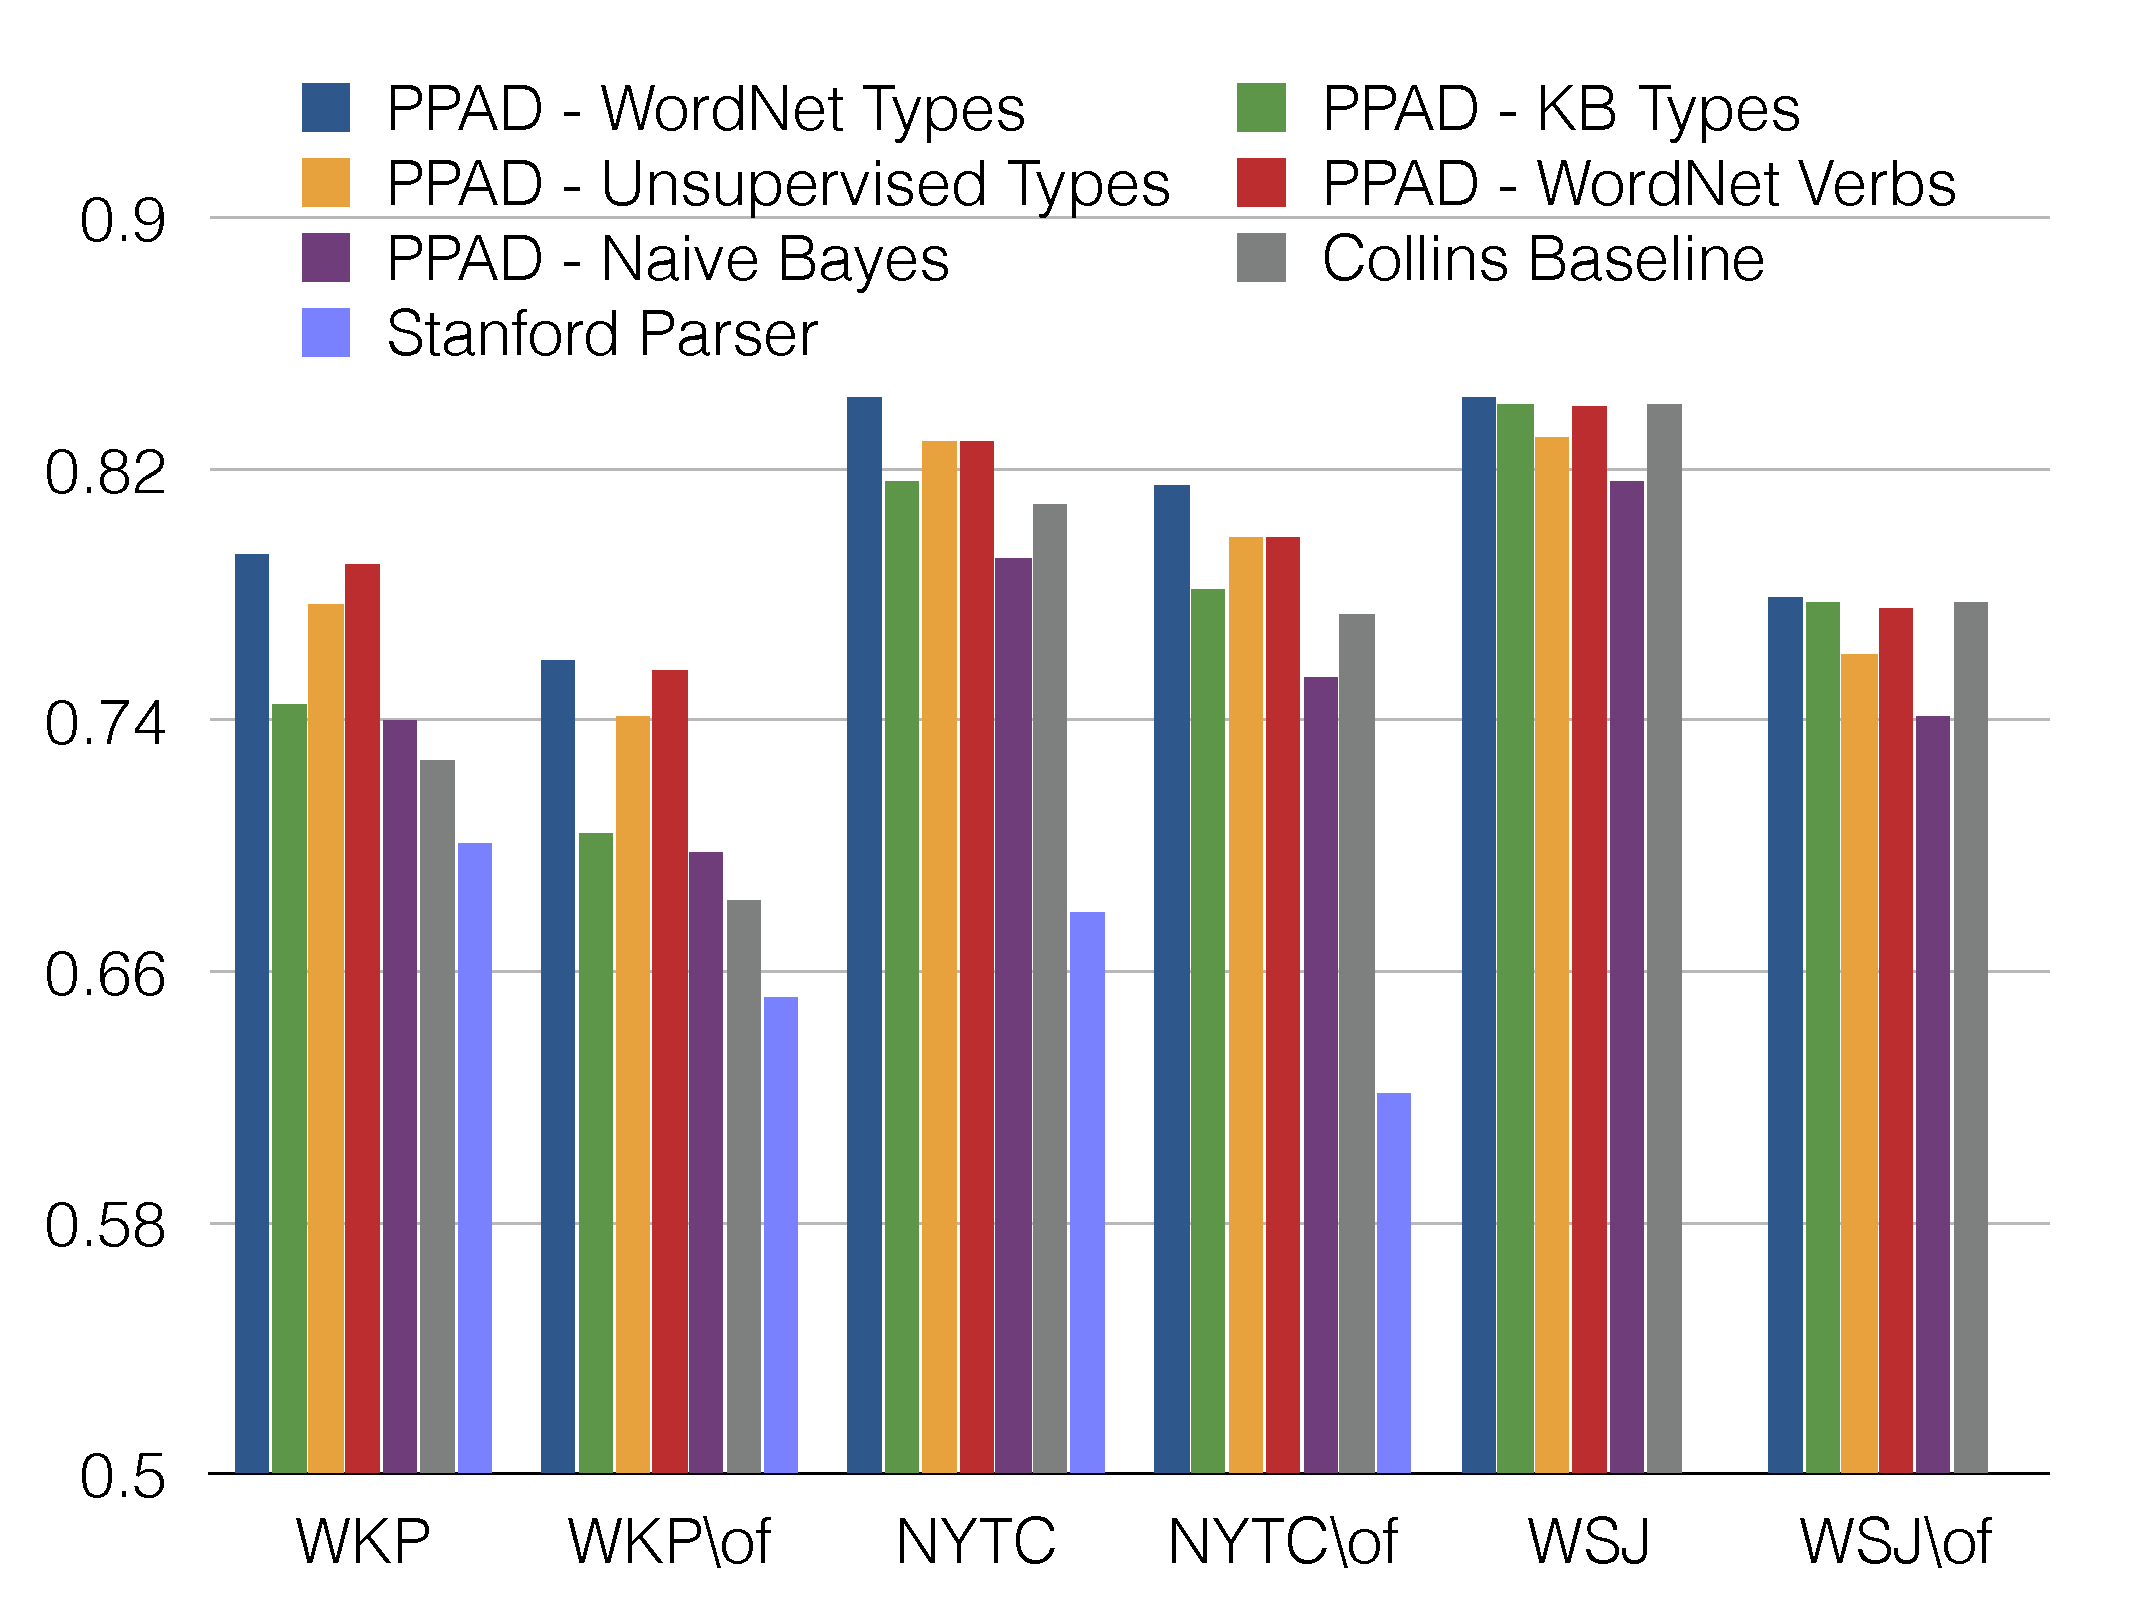
\includegraphics[width=1\columnwidth] {mainresults-2.pdf}
%
\vspace*{-1cm}
\caption{PPAD variations vs. baselines.}
%
\label{fig:resultmain2}
%
\end{figure}
    
   
    
 \paragraph{Methods Under Comparison} 
\textit{1) PPAD}  (Prepositional Phrase Attachment Disambiguator) is  our proposed method. It uses diverse types of semantic knowledge, a mixture of labeled and unlabeled data for training data, a logistic regression classifier, and expectation maximization (EM) for parameter estimation \textit{2) Collins} is the established baseline among PP attachment algorithms \cite{Collins95}.  \textit{3) Stanford Parser} is a state-of-the-art dependency parser, the 2014 online version. \textit{4) PPAD Naive Bayes(NB)}  is the same as PPAD but  uses a generative model,  as opposed to the discriminative model used in  PPAD.


 \subsubsection{PPAD vs. Baselines}
Comparison results of our method to the three baselines are shown in Table \ref{fig:resultmain}. For each dataset, we also show  results when the ``of" quads are removed, shown as ``WKP\textbackslash of'', ``NYTC\textbackslash of'', and ``WSJ\textbackslash of''.
 Our method yields  improvements over the baselines. Improvements are  especially significant on the datasets for which no labeled data was available  (NYTC and WKP). On  WKP, our method is 7\% and 9\% ahead of the Collins baseline and the Stanford parser, respectively.  On  NYTC, our method is 4\% and 6\% ahead of the Collins baseline and the Stanford parser, respectively. On WSJ, which is the source of the labeled data, our method  is not significantly  better than the Collins baseline. We could not evaluate the Stanford parser on the  WSJ dataset.  The parser requires well-formed sentences which we could not generate from the WSJ dataset as it was only available to us in the form of  PP quads with no other sentence information.  For the same reason,  we could not generate discourse features,$F7$, for the  WSJ PP quads.  For the  NYTC and WKP datasets, we generated well-formed short  sentences containing only the PP quad and the noun preceding it.  

 
 \subsubsection{Feature Analysis}
We found that features $F2$ and $F6$ did not improve performance, therefore we  excluded them from the final model, PPAD. This means that binary noun-noun relations were not useful when used permissively, feature $F2$, but when used selectively, feature $F1$, we found them to be useful. Our attempt at mapping prepositions to  verb definitions produced some noisy mappings, resulting in feature $F6$  producing mixed results.
To analyze the impact of the unlabeled data, we inspected the  features and their weights as produced by the PPAD model. From the unlabeled data, new  lexical features were discovered  that were not in the original labeled data.   Some sample  new features with high weights for verb attachments are: \textit{ (perform,song,for,*), %(*,independence,from,*),
(lose,*,by,*),  (buy,property,in,*)}. And for noun attachments: \textit{(*,conference,on,*), (obtain,degree,in,*), (abolish,taxes,on,*).} 
  %These newly discovered features could be the reason PPAD performs better than baselines on corpora for which no labeled data was available.


We evaluated several variations of PPAD, the results are shown in 
Figure \ref{fig:resultmain2}. For ``PPAD-WordNet Verbs",  we expanded the data by  replacing verbs in PP quads with synonymous WordNet verbs, ignoring verb senses.  This resulted in more instances of features F1, F8-10, \& F12. 

We also used  different types of noun categorizations: WordNet classes, semantic types from the NELL
knowledge base \cite{MitchellCHTBCMG15} and unsupervised types.  The KB types and the unsupervised types did not perform well, possibly due to the noise found in these categorizations.  WordNet classes showed the best results, hence they were used in  the final PPAD model for   features F3-4 \& F7.  In Section \ref{experimentalsetup}, PPAD corresponds to the best model.
  
     
     
 \subsubsection{Discussion: The F1 Score of Knowledge}
Why did we not  reach 100\% accuracy? Should relational knowledge not be providing a much bigger performance boost than we have seen in the results?
To answer these questions, we characterize our features in terms  precision and recall, and  F1 measure of their knowledge sources in Table \ref{fig:knowledgef1}. A low recall feature means that the feature does not fire on many examples, the feature's knowledge source suffers from low coverage.  A low precision feature means that when it fires, the feature could be incorrect, the feature's knowledge source contains a lot of errors. 
  

\begin{table*}[ht]
%
\centering
%
\begin{tabular}{|l|l|l|l|}
\hline 
\textbf{Feature Type} & \bf{Precision}  & \bf{Recall} & \bf{F1}\\
\hline
Noun-Noun Binary Relations (F1-2) &$low$ & $high$ &  $low$\\
Noun Semantic Categories (F3-4) & $high$ & $high$& \bf{high}\\
Verb Role Fillers (F5) & $high$ & $low$ & $low$ \\
Preposition Definitions (F6) & $low$ & $low$  &$low$ \\
Discourse Features (F7) & $high$ & $low$ & \bf{high} \\
Lexical Features (F8-15) & $high$ & $high$ & \bf{high} \\
\hline
\end{tabular}
\caption{An approximate characterization of feature knowledge sources in terms of precision/recall/F1}
 \label{fig:knowledgef1}
\end{table*}  
  
From Table \ref{fig:knowledgef1}, the  noun-noun binary relation features $(F1-2)$ have low precision, but high recall.
This is because the SVO data, extracted   from the ClueWeb09 corpus, that we used as  our  relational knowledge source is very noisy but it is high coverage. The low precision of the SVO data  causes these features to be detrimental to performance.  Notice that when we used a filtered version of the data, in feature $F2$, the data was no longer detrimental to performance. However, the $F2$ feature is low recall, and therefore it's impact on performance is also limited. The noun semantic category features $(F3-4)$ have high recall and precision, hence it to be expected that their impact on performance is significant. The verb role filler features  $(F5)$, obtained from VerbNet  have high precision but low recall, hence their marginal impact  on performance is also to be expected. The preposition definition features $(F6)$  poor precision made them unusable.  The discourse features $(F7)$  are based  noun semantic types and lexical features ($F8-15$),  both of which have high recall and precision, hence they useful impact on performance. 

In summary, low precision in knowledge is detrimental to performance. In order for knowledge to make even more significant contributions to language understanding, high precision, high recall knowledge sources are required for all features types. Success in ongoing efforts in knowledge base construction projects, will make performance of our algorithm better.  

\subsubsection{Application to Ternary Relations} \label{ternary}
Through the application of ternary relation extraction,  we further tested PPAD's PP disambiguation accuracy and  illustrated its usefulness for knowledge base population.
%In particular,  we studied accuracy on PP-attachments that express tenary relations by extending binary relations with one more argument.
Recall that a PP  5-tuple of the form $\{n0, v, n1, p, n2\}$, whose enclosed PP   attaches to the verb $v$,  denotes a ternary relation with  arguments \textit{n0, n1, \& n2}.
Therefore, we can extract a ternary relation from every 5-tuple for which our method predicts a verb attachment.   If we have a mapping between verbs and binary relations from a knowledge base (KB), we can extend KB relations to ternary relations by augmenting the KB relations with a third argument $n2$. 


\begin{table*}[ht]
%
\centering
%

\begin{tabular}{lp{1.4cm}lp{5.8cm}}
\hline
{\bf  Relation} &  {\bf  Prep. } & {\bf  Attachment accuracy}   &{\bf Example(s) } \\
\hline
acquired
%\newline purchased \newline bought
& from  & \textbf{99.97}  
& BNY Mellon	\textit{acquired}	Insight 	\textit{from}	Lloyds.\\
% \newline  \small{U.S.	\textit{bought}	Alaska	\textit{from}		Russian Rmpire.} \\
%\newline \small{Boeing	\textit{bought}	Jeppesen	\textit{from}	Tribune Company.}
%\newline  \small{Carolina Panthers	\textit{acquired}	Mccown	\textit{from}	Dolphins.}\\
\hline
hasSpouse & in  & \textbf{91.54} & David \textit{married}	Victoria	\textit{in}	Ireland.  \\
%\newline \small{Potts	\textit{married}	
%Alden Brown	\textit{in}	civil ceremony.}
%\newline \small{Henry Tate	\textit{married} Jane Wignall	\textit{in}	1885.}\\
\hline
	worksFor  & as & \textbf{99.98} & 
%	\small{Hillyer	\textit{joined} Boston Symphony Orchestra \textit{as}	violinist.} \newline
Shubert	\textit{joined}	CNN	\textit{as}	reporter. \\
		\hline
playsInstrument   & with & \textbf{98.40}  & Kushner	\textit{played}	 guitar	\textit{with}	rock band Weezer. \\
%\newline \small{Frehley	\textit{played}	lead guitar	\textit{with}	Chad Kroeger.} \\
\hline
%	musicianpla- \newline ysinstrument & played & for & \textbf{81.71}  & \small{Forminoya	\textit{played}	violin	\textit{for}	Eleanor Roosevelt.} \newline \small{Chilton Price	\textit{played}	violin	\textit{for}	Louisville Orchestra.}  \\
%     \hline
\end{tabular}
  \caption{Binary relations extended to ternary relations by mapping to verb-preposition pairs in PP 5-
tuples. PPAD predicted verb attachments with accuracy \textgreater 90\% in all relations.}
   \label{tab:tenary}
  \end{table*}
      
 % and the relation is expressed by the verb $v$.
We considered four KB binary relations and their instances such as $worksFor(Tim Cook, Apple)$, from the NELL KB. We then took the collection of 4 million 5-tuples  that we extracted from Wikipedia. We mapped verbs in 5-tuples to KB relations, based on  significant overlaps in the instances of the KB relations, noun pairs such as $(Tim Cook, Apple)$ with the  $n0,n1$ pairs in the Wikipedia PP 5-tuple collection. We found that, for example,  instances of the noun-noun KB relation ``worksFor" match $n0,n1$ pairs in tuples where  $v= joined$ and  $p=as$ , with  $n2$ referring  to the job title.  Other binary relations extended are: ``hasSpouse" extended by ``in" with wedding location, ``acquired" extended by ``from" with the  seller of the company being acquired.  Examples are  shown in Table \ref{tab:tenary}. 
In all these mappings, the proportion of verb attachments in the corresponding PP quads is significantly  high ( $ > 90\%$). PPAD is overwhelming  making the right attachment decisions in this setting.

Efforts in temporal and spatial relation extraction have shown that higher N-ary relation extraction is challenging.  Since prepositions specify details that transform binary relations to higher N-ary relations, our method can be used to read information that can augment  binary relations already in KBs. As future work, we would like to incorporate our method into a pipeline for reading beyond binary relations. One possible direction is to read details about the \textit{where,why, who} of events and relations, effectively moving from extracting only binary relations to reading at a more general level.


\subsubsection{Labeled Ternary Arguments}
In the above experiment, we studied the case of extending existing KB relations to ternary relations
with a third argument. However, we did not have any semantic information about the role of the third arguments. In this section, we study a different case, the case when we want to label the role of the third argument. For example, for the acquisition instance of ``BNY Mellon acquired Insight from Lloyds",  we want to predict that the label of ``Lloyds" is the ``Source",  indicating the source company of acquisition.  As another example, consider the buy instance `Bailey	bought	earrings	for	Josie",  we want to predict that the label of ``Josie" is ``Beneficiary", indicating the beneficiary of the earrings bought. 

To obtain labels for third arguments, we make use of VerbNet \cite{KipperKRP08}. VerbNet provides, for each verb, frames of the different use cases of the verb. Here we consider only  verb uses  that make use of prepositions. In VerbNet, these frames are described using a  label of ``primary=NP V NP PP.label" where the ``label" is the role of the third arguments following the prepositional phrase. One example is ``primary=NP V NP PP.instrument", each such frame is accompanied by an example sentence. In this case the example is: ``Paula hit the ball  with a stick", where the ``stick" takes the role of the instrument. Notice  that a given  verb and preposition combination does not necessary invoke a given label. For example in ``Paula hit the ball with joy", ``joy" does not play the role of the instrument. Therefore,  we learn introduce further constraints. We learn these constraints from the collection of 4 million 5-tuples  that we extracted from Wikipedia as explained in Section \ref{experimentalsetup}. In particular, we  replace mentions of entities with their NELL and WordNet semantic types. Using this approach, we generate templates of the form:
  \begin{table}[h]
  %
 \centering
  %
     \begin{tabular}{ll}
       \hline
\textless np\_v\_np\_pp.LABEL \textgreater \textless verb\textgreater \textless typeofArg1\textgreater \textless preposition \textgreater \textless typeofArg2\textgreater \\
            \hline
     \end{tabular}
       \label{tab:ternarylabels}
     \end{table}
    

We worked with five labels from VerbNet: 
np\_v\_np\_pp.beneficiary, np\_v\_np\_pp.instrument,\\ np\_v\_np\_pp.asset,
 np\_v\_np\_pp.source, and  np\_v\_np\_pp.topic. 
 Examples of learned templates for each of the five labels are as shown below in Table \ref{tab:ternarylabelsTemplates}.
 \begin{table}[h]
  %
 \centering
  %
     \begin{tabular}{ll}
       \hline
       
\textless np\_v\_np\_pp.beneficiary \textgreater \textless buy\textgreater \textless jewelry\textgreater \textless for \textgreater  \textless person\textgreater \\
 
\textless np\_v\_np\_pp.instrument \textgreater \textless shoot\textgreater \textless person\textgreater \textless with \textgreater \textless weapon\textgreater \\

\textless np\_v\_np\_pp.asset \textgreater \textless sell\textgreater \textless company\textgreater \textless for \textgreater \textless amount\textgreater \\

\textless np\_v\_np\_pp.source \textgreater \textless buy\textgreater \textless organization\textgreater \textless from \textgreater \textless organization\textgreater \\

\textless np\_v\_np\_pp.topic \textgreater \textless ask\textgreater \textless person\textgreater \textless for \textgreater \textless advice\textgreater \\
  
  \textless np\_v\_np\_pp.topic \textgreater \textless ask\textgreater \textless person\textgreater \textless for \textgreater \textless divorce\textgreater \\
            \hline
     \end{tabular}
     \caption{Examples of learned templates for labeled ternary relations}
       \label{tab:ternarylabelsTemplates}
     \end{table}
     
Table \ref{tab:ternarylabels}  shows sample instances of the different learned  templates for labeled ternary arguments.
We randomly sampled 100 such instances evaluated them for accuracy, we found a sampling accuracy of 88\%.


  \begin{table}[h]
  %
 \centering
  %
     \begin{tabular}{ll}
        \hline
        Ternary argument label &  Instance \\
       \hline
 np\_v\_np\_pp.beneficiary &	danai udomchoke	won	gold medal	for	thailand	\\
%np\_v\_np\_pp.beneficiary	& ian epton	won	gold medal	for	south africa	 \\
np\_v\_np\_pp.beneficiary &	alton	cooked	breakfast	for	crew	 \\
np\_v\_np\_pp.beneficiary & 	boys	cooked	cakes	for	girls	 \\
%np\_v\_np\_pp.beneficiary & 	mama	buys	piggy bank	for	cubs	 \\
np\_v\_np\_pp.beneficiary &	bailey	buys	earrings	for	josie	 \\
%np\_v\_np\_pp.beneficiary &	resources	buys	merchandise	for	attendees	 \\
%np\_v\_np\_pp.beneficiary &	duncan busby busby	won	gold medals	for	england	 \\
np\_v\_np\_pp.beneficiary &	jim	buys	bracelet	for	kathy	 \\
np\_v\_np\_pp.beneficiary &	leonard	buys	engagement ring	for	michelle	 \\
%np\_v\_np\_pp.beneficiary &	characters	buys	wine coolers	for	teenagers	 \\
np\_v\_np\_pp.beneficiary &	headmaster	bought	goggles	for	children	 \\
%np\_v\_np\_pp.beneficiary &	mayor bertrand-geslin	bought	collection	for	town	 \\
np\_v\_np\_pp.instrument &	lord edward thynne	shot	golden eagle	with	rifle	 \\
%np\_v\_np\_pp.instrument &	wahoo	opened	fire	with	mm guns	 \\
np\_v\_np\_pp.instrument &	mohawks	opened	fire	with	gunshots	 \\
%np\_v\_np\_pp.instrument &	portuguese garrison	opened	fire	with	artillery	 \\
np\_v\_np\_pp.instrument &	unidentified militants	opened	fire	with	grenade launcher	 \\
np\_v\_np\_pp.instrument &	jarvis	opened	fire	with	5-inch guns	 \\
np\_v\_np\_pp.instrument &	prince	stabs	vizier	with	dagger	 \\
np\_v\_np\_pp.instrument &	isaac van scoy	killed	british soldier	with	pitchfork	 \\
np\_v\_np\_pp.instrument &	ambush positions	opened	fire	with	mortars	 \\
np\_v\_np\_pp.instrument &	tamalika karmakar	killed	rebecca	with	knife	 \\
%np\_v\_np\_pp.instrument &	u-185	opened	fire	with	aa guns	 \\
np\_v\_np\_pp.source & telugu film homam	drew	inspiration	from	martin scorsese \\
np\_v\_np\_pp.source&	john coltrane	received	call	from	davis	 \\
np\_v\_np\_pp.source&	kenneth o'keefe	received	letter	from	state department	 \\
np\_v\_np\_pp.source&	tony	receives	letter	from	mandy	 \\
%np\_v\_np\_pp.source&	daughter	bought	tie	from	school	 \\
np\_v\_np\_pp.source&	peter	receives	call	from	claire	 \\
np\_v\_np\_pp.source&	huppertz	drew	inspiration	from	richard wagner	 \\
np\_v\_np\_pp.source&	fiz	receives	call	from	alan hoyle	 \\
np\_v\_np\_pp.source&	elbaz	drew	inspiration	from	bruce willis	 \\
np\_v\_np\_pp.source&	smolensky	bought	company	from	wheeler	 \\
n %p\_v\_np\_pp.topic&	marston	asks	marshall	for	help	 \\
%np\_v\_np\_pp.topic&	dead woman	asked	jack harper	for	help	 \\
np\_v\_np\_pp.topic&	wittenberg	asked	jan kazimierz	for	permission	 \\
np\_v\_np\_pp.topic&	brando	asked	john gielgud	for	advice	 \\
np\_v\_np\_pp.topic&	lutician delegates	asked	conrad	for	help	 \\
%np\_v\_np\_pp.topic&	doggett	asks	hayes	for	help	 \\
%np\_v\_np\_pp.topic&	marshall	asks	barney	for	advice	 \\
np\_v\_np\_pp.topic&	logan	asked	scott	for	help	 \\
%np\_v\_np\_pp.topic&	insult comic dog	asks	lopez	for	permission	 \\
np\_v\_np\_pp.topic&	philadelphia quakers	asked	nhl	for	permission	 \\
%np\_v\_np\_pp.topic&	hume	asked	john paul ii	for	permission	 \\
%np\_v\_np\_pp.topic&	hallman	asked	ncaa	for	permission	 \\
%np\_v\_np\_pp.topic&	countless times	asked	user	for	help	 \\
np\_v\_np\_pp.topic& steven	asks	frank	for	advice	 \\
%np\_v\_np\_pp.topic&	clerk	asks	peter	for	help	 \\
%np\_v\_np\_pp.topic&	commander wheeler	asks	hatfield	for	permission	 \\
%np\_v\_np\_pp.topic&	linden	asks	holder	for	help	 \\
np\_v\_np\_pp.topic&	rowe	asked	jackson	for	divorce	 \\
            \hline
     \end{tabular}
     \caption{Sample instances of    templates learned for labeled ternary arguments. For each instance, the label applies
     to the last argument.}
       \label{tab:ternarylabels}
     \end{table}

\subsection{Prepositional Phrase Attachment Ambiguity  Summary}
We have presented a knowledge-intensive  approach to prepositional phrase (PP) attachment disambiguation, which is  a type of syntactic ambiguity. Our method incorporates  knowledge about verbs, nouns, discourse, and noun-noun binary relations.   We trained a model using labeled data and unlabeled data, making use of expectation maximization for  parameter estimation.
% Future work includes using our method in  higher-nary relation extraction.
Our method can be seen as an example of tapping into a positive feedback loop for machine reading, which has only become possible in recent years due to the progress made by  information extraction and knowledge base construction techniques.


 
 

%\section{Event Extraction}
% Binary relations are well-studied, higher-nary ones are not.
% 

Developing techniques for higher-nary relation extraction  is a natural next step  after  the well-studied case of binary relations \cite{Auer07,suchanek2007yago,Bollacker2008,Carlson2010,MitchellCHTBCMG15}.  
  %This has resulted in a triple  fact that many relations are expressed as  assuming that   binary relations are expressed as triples of the form,
  In the literature, prominent  binary relation extraction methods  are mostly  semi-supervised \cite{Suchanek:2009,Carlson2010} or  unsupervised  \cite{Mausam2012,fader2011identifying}. Semi-supervised methods tend to have higher precision than unsupervised methods and therefore are commonly used to populate knowledge bases  of facts \cite{Nakashole2011,MitchellCHTBCMG15}. In such settings,  relations of interest are predefined, i.e, company acquisitions or  protein-protein interactions.
However,  in semi-supervised approaches,  one needs to provide seed examples for each relation to bootstrap the extractor. This can be expensive, especially if there are many relations of interest. For ternary relations, hand specifying training instances per relation  requires even more time since each training instance is a triplet of three entities as opposed to a pair of entities for binary relations.  Most people know that Google acquired Youtube but not the dollar amount or the date of the acquisition, and most people know that Hillary Clinton is married to Bill Clinton by not the location or date of their wedding. This makes ternary training data generation  a  time consuming exercise in searching the Web. 
 
In this paper we present a resource  for training  ternary extractors. The resource was generated using a minimally supervised yet  high precision method.
% method for generating training instances for  ternary relations, which only requires minimal supervision. 
%Towards this end, we   exploit
% language structure
% in building higher-nary relation extractors.
% much like binary relation extractors have leveraged language structure \cite{Fader2011}.
%One obvious kind of language construction that extract ternary relations is 
Our method leverages a very common language construction: prepositional phrases (PPs).   PPs such as  ``in X", ``at Y", and ``for Z" express details about the  \textit{where, when,} and \textit{why}  of  binary relation instances. This makes PPs well-suited to extending binary relations by one more argument, extending them to ternary relations.
 
 Consider the following occurrences of 5-item sequences of the form: N1, V, N2, P, N3; where the Ns are noun phrases,  V is a verb and P is a preposition.
 \begin{table}[h]
    \small{
 \centering
 \begin{tabular}{p{7cm}}
 \textit{(1) \textbf{Mercedes-Benz}	bought	\textbf{Chrysler}	for	\textbf{\$40 billion}}\\
  %\textit{Microsoft	acquired	Chrysler	for	\$500 billion}\\
   \textit{(2) \textbf{CBS}	bought	\textbf{WCCO}	from	\textbf{General Mills}}\\
 % \textit{(2)Wolkswagen AG	bought	Auto Union GmbH	from	Daimler Benz}\\
% \hline
% \textit{(3) Suzanne Somers	sued	ABC	for	\$ 2,000,000.}\\
% \textit{(4) Alexandroni Brigade	sued	Teddy Katz	for	libel}\\
  \hline
  \textit{(3) \textbf{Joe Lieberman}	endorsed	\textbf{McCain}	for	\textbf{president}}\\
  \textit{(4) \textbf{The New Yorker}	endorsed	\textbf{Obama}	over	 \textbf{Romney}}\\
 \end{tabular}
 \label{tbl:example}
 }
 \end{table}

In a large Web extracted corpus, one sees many 5-item sequences similar to each of the 6 types shown above. The verbs and prepositions do not change but the arguments N1-3 change. From a large volume of such occurrences, we can learn templates for populating ternary relations. For example, from many occurrences of tuples of type (1), we can generate the template:   \textit{ \textless organization\textgreater	bought \textless organization\textgreater	for	\textless dollar\_amount\textgreater}. We go further by having labels for all three argument placeholders.  For this particular template the labels are: \textit{AcquisationEventAcquirer, AcquisationEventAcquired, AcquisationEventAmount} for the N0, N1, N3, argument placeholders respectively.
Similarly, from tuples of type (3), we can generate the template:   \textit{ \textless person\textgreater	endorsed \textless politician\textgreater	for	\textless political\_office\textgreater}. And the corresponding argument labels are: \textit{EndorsementEventEndorser,	EndorsementEventEndorsed,	EndorsementEventOffice}, for the N0, N1, N3 argument placeholders respectively. A triplet of argument labels is considered to be a ternary relation. And matching triplets of entities are considered to be instances of ternary relations.

In summary, the contributions of this paper are twofold:

\textit{1)~ Resource:}  A resource for boostrapping ternary relation extraction. It contains ternary relations and their instances. It also contains templates used to populate ternary relations. We make the data available for future research. It is also attached as supplementary data to this submission.
%triplets of entities
% (e.g. ( Joe Kieberman, John McCain, president), labeled with their argument roles for specific ternary relations (e.g, (EndorsementEventEndorser,	EndorsementEventEndorsed,	EndorsementEventOffice)). For each triplet, the resource specifies the template used to generate it.

\textit{2)~ Data Generation Method:} We describe  the approach used to generate this resource, which others can replicate to generate similar resources in their  domains of interest.

 %NEL_organization	endorsed	NEL_person	over	NEL_person
 
% cbs	bought	wcco	from	general mills
% u.s.	bought	alaska	from	russia
% olkswagen ag	bought	auto union gmbh	from	daimler benz
%
%johnson	acquired	neutrogena	for	$ 924 million
%microsoft	acquired	hotmail	for	$ 500 million
%mercedes-benz	buys	chrysler	for	$ 40 billion

%HiringEvent	NEL_organization	appointed	NEL_person	as	NEL_profession	143	HiringEventHirer	HiringEventHiree	HiringEventPosition

% For example, binary extractors have used the assumption that the majority of binary relation types can be expressed by verb phrases. And therefore, prominent binary relation extraction methods extract relation instances by analyzing triples of the form  noun-verbphrase-noun \cite{Fader2011,Nakashole2011,Nakashole:2012:Patty}.

%AcquisitionEvent	NEL_organization	acquired	NEL_person	from	NEL_organization	156	AcquisationEventAcquirer	AcquisationEventAcquired	AcquisationEventSeller
%AcquisitionEvent	NEL_organization	bought	NEL_organization	for	<nell_amount>	38	AcquisationEventAcquirer	AcquisationEventAcquired	AcquisationEventAmount
%AttackEvent	NEL_organization	fired	NEL_weapon	at	NEL_organization	37	AttackEventAttacker	AttackEventInstrument	AttackEventAttacked
%DefeatEvent	NEL_sportsteam	defeated	NEL_sportsteam	in	NEL_event	189	DefeatEventVictor	DefeatEventDefeated	DefeatEventOccasion
%
%HiringEvent	NEL_person	appointed	NEL_person	as	NEL_profession	182	HiringEventHirer	HiringEventHiree	HiringEventPosition
%
%MeetingEvent	NEL_person	met	NEL_person	in	NEL_location	135	MeetingEventPerson1	MeetingEventPerson2	EventLocation
%
%SuingEvent	NEL_person	sued	NEL_organization	for	WDN_discourtesy	22	SuingEventSuer	SuingEventSued	SuingEventReason
%
%SuingEvent	NEL_person	sued	NEL_organization	for	<nell_amount>	20	SuingEventSuer	SuingEventSued	SuingEventAmount
%
%WeddingEvent	NEL_person	married	NEL_person	in	NEL_location
%WeddingEvent	NEL_person	married	NEL_person	in	<nell_date>


% where the relations of interest are predefined.
%The way semi-supervised methods work is by starting with a few seed instances for each relation. A large corpora is then used to find sentences which contain these instances, thereby generating training sentences for machine learning classifiers. These classifiers  learn to predict which patterns are good indicators of mentions of seeded relations.

% In the OpenIE and supervised IE, distant supervisio with have been found to be used.
%  OpenIE, and semi-supervised methods, 

%Boostraping methods are about starting with a few seeds to populate relations. How is boostrapping done.
%
% The problem is that  PPs are a major source of  syntactic  ambiguity, they have been found to be causing  most  parsing errors across many parsers (biggest contributor).
% \highlight{What is the problem caused by PPs? They are usually treated as v p n. Show a tree, with useful ternary relations that can fill a KB. Tell that in the case of V, we have a ternary relation, in the case of N, we have a binary relation}, here we are interested in 5-tuples, not quads.
% 
%  In this paper, we study how PPs would affect a PP-based ternary extractor. Would we extract ternary relations that should really be binary relations (assuming V attachment instead of N attachment? ), in the general case, this is expected to be Yes. For the typical verbs that are in knowledge bases, is this an issue?? the answer is yes, because PP exist. So we look into these verbs, in particular, common relations of interest. What happens when we employ typing, we type the arguments. 
%  
  
  \subsection{Related Work}
  To supervise binary relation extraction methods,  there is an abundance  of resources. Knowledge bases (KBs) such as  DBPedia \cite{Auer07}, YAGO \cite{suchanek2007yago}, Freebase\cite{Bollacker2008}, and NELL \cite{MitchellCHTBCMG15}, as well as Open IE tools and resources such as Reverb \cite{Fader2011}, and Ollie \cite{Mausam2012} contains many millions of binary relation instances that can be used  to distantly train binary relation extraction. However, these knowledge bases are highly impoverished when it comes to ternary relations.  In contrast, we provide a resource that can be used directly to train and encourage more research on the higher-nary machine reading and relation extraction. A number of works have studied temporal scoping of  facts by adding a time dimension to facts \cite{wang2010timely,wijayactp}. While temporal scope generates ternary relations, for example by using reification, this only deals with one type of ternary relation. In contrast, our resource contains $50$ ternary relations, spanning $18$ high level topics or  event types.
  
  \begin{table}[t]
  \begin{tabular}{|l|l|}
  \hline
  ElectionEvent & AwardEvent \\
  HiringEvent & FiringEvent \\
  AcquisitionEvent & WeddingEvent \\
  DivorceEvent & DefeatEvent \\
  MeetingEvent & AttackEvent \\
  ProductLaunchEvent & EarthquakeEvent \\
  MurderEvent & PerformingEvent \\
  SuingEvent & BombingEvent \\
  EndorsementEvent & ShootingEvent \\
  \hline
  \end{tabular}
  \caption{Event types (18) or high level topics in our resource.  The resource contains 50 ternary relations across these topics.}
  %For each event type, the method generates relevant ternary relations, as many as can be found in the input raw corpus. We found a total of $50$ ternary relations across the $18$ event types/topics.}
  \label{eventtypes}
  \end{table}
  
 \subsection{Data Generation}
In this section we present our method for generating the ternary relations and their instances.

\subsubsection{Input}
As input, our method takes a natural language text corpus and   high level topics or even types of interest. Our method automatically learns many different ternary relations relevant for each event type. There are two advantages to  specifying event types of interest instead of directly thinking in terms of  ternary relations.  First, a broad event type can capture many relevant ternary relations that naturally appear in the data. Second, it requires much less human effort to specify one event type than manually specifying a list of all conceivable  ternary relations, some of which might not be present in the data.

Table \ref{eventtypes} shows the event types covered in our resource. For each event type, we specified at most three \textit{trigger verbs} that indicate a potential mention of the event type. We will later describe how to automatically extend  event trigger verbs in an iterative manner. This is done in a similar way to extending seed instances or patterns of  binary relations \cite{Suchanek:2009,Nakashole2011,MitchellCHTBCMG15}.



\subsubsection{Candidate Template Generation} \label{candidates}
Once we have event types defined with their trigger verbs, we can  generate ternary relations
for each event type. The first step is to generate ternary relation \textbf{templates}. An example template is: \textit{ \textless person\textgreater	endorsed \textless politician\textgreater	for	\textless political\_office\textgreater}.  We generate these templates directly from the data. We do this by first parsing the raw corpus, and extracting 5-item sequences of the form:  N1, V, N2, P, N3; where the Ns are noun phrases,  V is a verb such that V is a trigger verb of one of the events,  and P is a preposition.
We generate templates from 5-item sequences as follows: we replace every noun phrase N1-N3 by its semantic type.
In particular, we do lookups of entity types in two types of semantic hierarchies, WordNet and the NELL type hierarchy \cite{Carlson2010}. We found the two type systems to be complementary: WordNet contains more common nouns whereas NELL contains more proper nouns.
Our generated templates can therefore contain a mixture of WordNet types and NELL types. For example, for the \textit{MurderEvent}, the following is a valid template that our approach generated: \textit{\textless NEL\_person\textgreater	killed	\textless NEL\_person\textgreater	with	\textless WDN\_weapon\textgreater}. The semantic types in our templates are prefixed by three letters, \textit{NEL} for NELL types, and \textit{WDN} for WordNet types.

We retain, as candidate templates, all the templates of the form:
\textit{\textless N1\_type\textgreater	V	\textless N2\_type\textgreater	P	\textless N3\_type\textgreater}, whose support size is $>=3$. That is, the template was generated from three or more  5-item sequences, N1, V, N2, P, N3, with distinct noun arguments (N1-N3).

\subsubsection{Template Filtering}\label{filteringandinstances}
From the candidate templates, a final set of templates is generated.
To do this, we manually filter out all templates that do not express useful
ternary relations for the topic at hand. Once we have filtered out the templates, for each
template, we manually label each template with  descriptive labels for the its corresponding 
noun phrase placeholders. For example, \textit{\textless NEL\_person\textgreater	killed	\textless NEL\_person\textgreater	with	\textless WDN\_weapon\textgreater} is labeled with \textit{MurderEventMurderer, MurderEventMurdered, MurderEventInstrument}. Each triple of labels is considered to  be a single \textbf{ternary relation}. Therefore we have the ternary relation \textit{Murderer\_Murdered\_Instrument}. Such a ternary relation would  has \textbf{instances} such as \textit{Bob,Alice,knife},  which indicates that Bob murdered Alice with a knife.

We obtain instances of templates, and hence ternary relations, by  retaining the supporting 5-item sequences of each of the accepted templates.
%The sequences are considered to be \textit{instances} of ternary relations, where each ternary relation
%is defined by a template
 Notice that each instance  has labeled noun phrases  because the instances inherit  argument labels from their templates.
 
 
It is worth noting that  template filtering is the part requiring the most manual supervision. All the other parts are automated.  While, the specification of event types and their trigger verbs is also manual, it is quite fast, requiring only up to three trigger verbs per event type.  


% \highlight{This is now a dataset presentation paper. We make sure that we have no methodology section. Additionally, we present the first dataset, then we present the first dataset plus iteration 1, then first dataset plus first 5 iterations. From each randomly sample 100 templates that were not generated. Tell the people we make available, our templates, and the instances that can be used as training data for higher n-nary systems. Our data set was generation semi-automatically.}
% The boostrapping approach for binary relations looks like this \cite{Hearst92}.
% We are interested in 
 
 \subsubsection{Iterative Template Generation} \label{iterate}
 In order to extend the size of the resource, we  increase the number of trigger verbs per event type. We  do this automatically. First, from the raw data, we extract 5-item sequences of the form $N1, V, N2, AP, N3$. There are two main differences between these sequences and the 5-item sequences we have worked with up to now. First,  here $V$ is any verb, not limited to the trigger verbs that were manually specified. Second, we no longer limit the phrase between $N2$ and $N3$ to prepositional phrases, $P$ is now $AP=any$ $phrase$. We limit the length of $AP$ to a maximum of three words.  
 We then find 5-item sequences where all three arguments $N1-3$ match the arguments of an instance of a template from Section~\ref{filteringandinstances}.  Thus, we are using the instances generated so far as distant supervision to discover new templates. 
 
 All new $(V,AP)$ pairs forming candidate templates that occur with more than $10$ distinct instances of an existing template qualify  a new promoted  templates. We increase the minimum support required from $3$ to $10$ to avoid introducing noisy templates.
A new template has  the same argument role labels as the original template whose instances overlap with the instances of the new template.  This process extends the trigger verbs, and is not  limited to prepositions for the extraction of the third argument.   This also allows the generation of more instances from the newly discovered templates. Notice that the number of ternary relations  remain constant from the initial template generation step where we manually label templates with argument roles.
 %This process also increases the  number of  instances from the new templates.
 %, as we can use the new template to extract instances of the corresponding ternary relation.
 % analogous to the case of binary relations \cite{Hearst92}.
 

%\section{Resource Quantitative Analysis}
%We present statistics on the size and quality of the resource,
%
%\highlight{1)In resource: trigger verbs.tsv}\\
%\highlight{2)Iorbittn resource: instances of templates.tsv}\\
%\highlight{3)In resource: templates only.tsv}\\


\subsection{Evaluation}
We applied our data generation process to  Wikipedia (WKP) and the  ClueWeb09 (CWB) corpus. 
We first generated an initial set of candidate  templates from Wikipedia, using the method described in Section \ref{candidates}. We did not apply this step to the ClueWeb corpus as it can be noisy. We then manually filtered the generated candidate templates as described in Section \ref{filteringandinstances}. This is  iteration $0$. We had a total of $186$ templates at iteration $0$, and  $50$ ternary relations across $18$ event types.  The number of templates increase across iterations.
%but the number of ternary relations remain the same.
 Therefore, in subsequent iterations, we obtain more templates that can be used to populate our $50$ ternary relations. 

 From the  initial templates, we generate template instances both from Wikipedia and the ClueWeb corpus. These are triples of entities whose types match the argument types of the template, and they occur with the lexical items that appear in the template. We then use the instances as distant supervision to generate more templates as described in Section \ref{iterate}. Again, we only discover new templates from Wikipedia, using only ClueWeb to find instances for the discovered templates. At iteration 1, we discovered an additional 174 templates.
 
 Our method picked up new templates until iteration 3, making a total of $502$ templates. Figure \ref{fig:templates} shows the cumulative number of templates across iterations. Also shown in Figure \ref{fig:templates}  is precision of templates.  We manually assessed precision at every iteration, we did this by randomly selecting $100$ templates discovered at every iteration, or all templates if less than $100$ templates were discovered in a given iteration. Precision is $100$\%  at all iterations, except for iteration 2 where it dropped to $95$\%. 
This was due to a   few cases of semantic drift not being cutoff by thresholds of our methods. This led our method do discover templates with verbs such as ``resigned as" in templates associated with \textit{hiring} events, we marked these as wrong.

Figure \ref{candidates} shows the cumulative number of instances picked up at every iteration. We started with $31,161$ from WKP and CWB corpora at iteration $0$ and ended up with $61,380$ instances  by the third and final iteration. This number could be increased by 1) allowing discovery of templates from the ClueWeb corpus or other large corpora 2) lowering the high thresholds on the minimum support size of learned templates .
Since  instances are generated from templates, their precision can be   inferred from the precision of the templates. To a small extent, instances can also contains errors  stemming  from:  noun phrase chunking and  semantic types; these  errors can be fixed by using  accurate better chunkers  and semantic typing systems.
% For each instance, we keep track of the template(s) that were used to generate it.

\begin{figure}[t]
 %
 \centering
 %
 \includegraphics[width=0.80\columnwidth] {template-precision.pdf}
 \vspace*{-0.98cm}
 \caption{Precision and accumulated number of learned templates, iterations $0-3$}
 \label{fig:templates}
 %
 \end{figure}  
 

 \begin{figure}[t]
  %
  \centering
  %
  \includegraphics[width=0.80\columnwidth] {instance-recall.pdf}
  \vspace*{-0.4cm}
  \caption{Accumulated number  of instances.}
  \label{fig:instances}
  %
  \end{figure}  
%
%\begin{itemize}
%\item First look at performance when the arguments of the  PPs are not typed, what happens 
%when we just say verb, P, N1, N2: when the verbs are not typed.
%\item Second, look at performance when the 
%\end{itemize}


%
%\begin{itemize}
%\item Prepositional sense disambiguation is not what we are after
%\item Methods for information extraction from prepositions: Look into this.
%\item Work in temporal relation extraction can be formulated as ternary relation extraction but it is only one particular type of relation.
%\item Open IE, still also will suffer from PP.
%\item Semantic role labeling, the issue is that PPs are ignored in state of the art semantic role labelling such as semafor, and are not adequately tackled.
%\end{itemize}



\subsection{Events Summary}
In this paper our goal is to address the  bottleneck that has throttled research in higher n-ary relation extraction. To this end, we generated a training data resource for ternary relation extractors.  We described a method for learning and populating ternary relations initially only  using prepositional phrase based templates. Additionally, our method  also learns templates that are not based on prepositions, in an iterative manner. We hope this resource  encourages  research on ternary relation extraction. 
\clearpage
\section{Compound  Nouns Analysis} \label{nominals}
The second example of a language construct that causes problems for machine reading in the absence of background knowledge 
arises from the use of compound nouns. Noun phrases contain a number of challenging compositional
phenomena, including implicit relations.
  Compound nouns such as ``pro-choice Democratic gubernatorial candidate
James Florio'', or ``White House spokesman Marlin Fitzwater'' primarily consist of  nouns and adjectives. They do not contain verbs. 
This means that it is difficult for a pattern detection algorithm to detect any useful lexical regularities across compound nouns that express the same relations.   On the other hand, beliefs such as a person’s job title, nationality, or stance on a political issue
are often expressed using compound nouns. We  propose a knowledge-aware algorithm for extracting semantic relations from compound noun analysis that learns, through distant supervision, to  map fine-grained type sequences of compound nouns to the relations they express.
Consider the following compound nouns. 



\begin{table}[h]
%
\centering
%
\begin{tabular}{ll}
\hline
1.a) Giants	cornerback	Aaron Ross \\
1.b) Patriots	quarterback	 Matt Cassel \\
1.c) Colts	receiver	Bryan Fletcher \\
\hline
2.a)  Japanese	astronaut	Soichi Noguchi \\
2.b) Irish	golfer	Padraig Harrington \\
2.c) French	philosopher	Jean-Paul Sartre \\
\hline
2.a) Seabiscuit	author	Laura Hillenbrand \\
2.b) Harry porter author J.K Rowling \\
2.c) Walking the Bible author Bruce Feile \\
\end{tabular}
%\caption{Example of nominals }
%\tom{What does "-" mean in this table?  If zero, let's use "0"}}
\label{tab:nominalsexamples}
\end{table}
     

The concepts in the  compound noun sequences \textit{(1a. -- c.)}, \textit{(2a. -- c.)}, \textit{(3a. -- c.)}  are
of the semantic type sequences:

\begin{table}[h]
%
\centering
%
 \begin{tabular}{ll}
   \hline
\textit{\textless sportsteam\textgreater \textless sportsteamposition\textgreater \textless athlete\textgreater}  \\
\textit{\textless country\textgreater \textless profession\textgreater \textless person\textgreater} \\
\textit{\textless book\textgreater  ``author" \textless person\textgreater} \\
        \hline
 \end{tabular}
 %\caption{Example of nominals }
 %\tom{What does "-" mean in this table?  If zero, let's use "0"}}
   \label{tab:nominalstypesequences}
 \end{table}
     
     

Therefore, our task is to learn semantic type sequences and their mappings to knowledge base relations. In our case we use relations from the NELL knowledge base. Since  NELL has   binary relations that  take only two arguments, and compound nouns contain more than two noun phrases,  we additionally keep track of the position information for the two arguments of the relation.  For example, from the type sequence:   \textit{\textless country \textgreater \textless profession\textgreater \textless person\textgreater}, we generate mappings to two different  relations.

\begin{table}[h]
\begin{tabular}{llll}
\hline
\textbf{Relation}&  \textbf{arg1\_pos} &  \textbf{arg2\_pos} & \textbf{type sequence} \\
\hline
citizenofcountry & 3 & 1 & \textit{\textless country\textgreater \textless profession\textgreater \textless person\textgreater} \\
personhasjobposition & 3 & 2 & \textit{\textless country\textgreater \textless profession\textgreater \textless person\textgreater} \\
     \hline
\end{tabular}
\caption{Learned mappings from compound nouns semantic type sequences to binary relations }
%\tom{What does "-" mean in this table?  If zero, let's use "0"}}
\label{tab:nominalsmappings}
\end{table}

\begin{figure}[t]
%
\centering
%
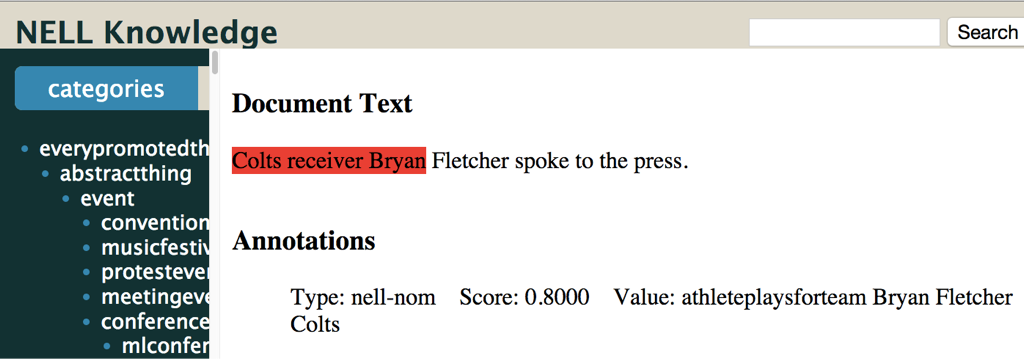
\includegraphics[width=1\columnwidth] {athletenominal.png}
%
%\vspace*{-1cm}
\caption{Extracting the athleteplaysforteam relation from a compound noun.}
%
\label{fig:athletenominal}
%
\end{figure}

To learn  mappings from  compound nouns to binary relations as shown in Table \ref{tab:nominalsmappings}, we  use  distant supervision, that is using the NELL knowledge base as the only form of supervision.   In general, the intuition behind
 distant supervision is that a sentence that contains a pair of entities that participate in a known
knowledge relation is likely to express that relation. In our case, the sentence is just a compound noun. Therefore, we first extract compound nouns from a large collection of documents.  For every compound noun,  we map its noun phrase to entities in the NELL. The entities are then replaced by their NELL types. This creates  type sequences of the form:  \textit{\textless country \textgreater \textless profession\textgreater \textless person\textgreater}.  Each type sequence has a support set, which is the collection of  compound nouns that satisfy the type sequence. For example, a support compound noun might be: \textit{Japanese	astronaut	Soichi Noguchi}   for the type sequence: \textit{\textless country\textgreater \textless profession\textgreater \textless person\textgreater}.  We retain type sequences whose support set sizes are above a threshold of  $10$ in our experiments.  For  type sequences with support set size above the threshold, we use their support sets to learn mappings from type sequences to relations using distant supervision.  That is, from each supporting compound noun we collect pairs of entities, and do look ups in NELL to determine which relations hold between the pair of entities. We additionally keep track of the position of  the entities within the compound noun. This gives us mappings from types sequences to relations such as:  \textit{\textless citizenofcountry\textgreater \textless3\textgreater  \textless1\textgreater \textless country\textgreater \textless profession\textgreater}. We only retain mappings that have a support set size (relation instances in NELL) above a threshold of $10$ in our experiments.

\subsection{Experimental Evaluation}
We extracted compound nouns from three different corpora: the New York
Times archive which includes about 1.8 Million
 articles from the years 1987 to 2007, the English edition of Wikipedia  with about
about 3.8 Million articles, and the KBP dataset \cite{conf/tac/Surdeanu13} which contains over 2 million documents with  Gigaword newswire  and Wb documents. We extracted a total of $2,270,487$ compound nouns.
From these compound nouns, we  extract 10 relations that are expressed by compound nouns and are in the NELL knowledge base. From this dataset we learned 291 mappings from  types sequences to relations.  Using these mappings we then predicted new relation instances. We report  recall and accuracy   in  Table \ref{tab:nominalsresult}. We can see that this approach has high accuracy across all the relations. Recall is also high for certain relations but low for others. This might be because  certain relations although they are expressed using compound nouns, they are more commonly expressed in other forms.

We have incorporated this system into the NELL reading software. A screenshot of extracting relations from compound nouns is shown in Figure \ref{fig:athletenominal}.



\begin{table}[h]
%
\centering
%
 \begin{tabular}{l|l|l}
 \hline
 Relation & Recall & Precision \\
   \hline
   citizenofcountry & 15,805 &$0.982\pm0.018$ \\
citylocatedincountry & 1,521 & $0.75\pm0.083$ \\
athleteplaysforteam &471 & $0.982\pm0.018$ \\
persongraduatedfromuniversity& 49 & $0.964\pm0.036$ \\
personhasjobposition & 511,937 & $0.837\pm0.07$ \\
musicianplaysinstrument & 3,890 & $0.885\pm0.06$ \\
worksfor & 75,757 &  $0.847\pm0.068$ \\
athletewinsawardtrophytournament & 92 & $0.928\pm0.049$ \\
coachesteam& 175 & $0.982\pm0.018$ \\
companysubsidiary& 37 & $0.953\pm0.047$ \\
   \hline
 \end{tabular}
 \caption{Recall and  precision of relation extraction for 10 relations. Precision is sampled
 from a total of max(100, recall).}
 %\tom{What does "-" mean in this table?  If zero, let's use "0"}}
   \label{tab:nominalsresult}
 \end{table}





    
\subsection{Related Work}
Much of the work on information extraction has been on extracting relations expressed by verb phrases
that occur between pairs of noun phrases. Extracting knowledge base relations from noun phrases alone has been much less
explored. In \cite{conf/emnlp/YahyaWGH14}, a method is  developed that learns noun phrase
structure for open information extraction. This is different from our work in that we are extract 
knowledge base relations as opposed to open information extraction. Therefore, the authors
do not ground their extracted attributes to an
external knowledge base. 


The work of \cite{choi2015scalable} developed a semantic parser for extracting relations
 from noun phrases. Given an input noun phrases, it is first transformed to a logical form, where the logical form is an 
 intermediate unambiguous representation of the noun phrase.
The  logical form is chosen such that it  closely matches the linguistic structure
of the input text noun phrase. The logical form is then transformed into one that, where possible,
uses the Freebase ontology predicates \cite{Bollacker2008}. These predicates can then be read off as relations expressed about the 
entities described by the noun phrase. The authors test their work on Wikipedia category names. Since each Wikipedia category
describes a set of entities, by extracting relations from each category name, one learns relations about all the members of the category.
Consider the Wikipedia category \textit{Symphonic Poems by Jean Sibelius}.  An example of the knowledge base transformed  logical form for this category name would be: 

$\lambda x.composition.form(x;Symphonic$ $poems) \wedge composer(Jean$ $Sibelius; x)$ where one can now extract attributes for the entities, such as \textit{The Bard, Finlandia, Pohjola’s Daughter, En Saga, Spring Song, Tapiola, \ldots},  that 
fall under this category  in particular that for all $x$ in this category $composer(Jean$ $Sibelius; x)$ and  $composition.form(x; Symphonic$ $poems)$
where $composer$ and $composition.form$ are Freebase attributes. In generating the logical forms, several features are used that capture some background knowledge, in particular,   a number of features that enable soft
 type checking on the  produced logical form, and  features that test agreement of these
 types on different parts of the produced  logical form.
 
In a related but different line of work,  the NomBank project  \cite{conf/lrec/MeyersRMSZYG04,conf/acl/GerberC10} annotated the argument
structures for common nouns. For example, from the expression \textit{Greenspan’s replacement Ben Bernanke},
the arguments for the nominal ``replacement", are: ``Ben
Bernanke" is  ARG0 and ``Greenspan" is  ARG1. The resulting annotations
has been used as training data for work on semantic role labeling on nominals \cite{jiang2006semantic,conf/acl/LiuN07}.
Again, this work is different from our work in that no knowledge base relations are extracted.


There has  also  work on the broader topic of semantic structure of noun phrases. In \cite{conf/acl/SawaiSM15}, a method is proposed that parsers noun phrases into the Abstract Meaning Representation in order to detect the argument structures, and noun-noun relations in compound nouns.


\subsection{Compound  Noun Analysis Summary}
We have presented a knowledge-aware method for relation extraction from 
compound nouns.   Our method uses semantic types of concepts in compound noun sequences
to predict relations expressed by novel compound noun sequences containing concepts that we have not seen before. This  method can be
seen as another example of tapping into a positive feedback loop for machine reading made possible by projects that construct large-scale knowledge bases. Compound nouns are non-trivial to interpret in many different ways besides the noun-noun relations problem we addressed here.  For example, one problem that could benefit from background knowledge is that of   analyzing the internal structure of noun phrases through bracketing \cite{conf/acl/VadasC07,conf/acl/VadasC08}.  For example, in the noun phrase \textit{(lung cancer) deaths},  the task would be to determine that  \textit{lung cancer} modifies the head \textit{deaths}. Additionally, as future work we can increase our predicate vocabulary to learn more common sense type of relations from compound nouns, for example, in the noun phrase \textit{cooking pot}, we can extract the relation\text{purpose}, to mean the pot is used for cooking.
 




\section{Discussion and Conclusion}\label{conclusions}
%Our experience with developing machine reading systems with access to high volume
%memory shows  the promise of this approach. In particular,
In this paper, we presented results on two cases studies of using background knowledge: firs,t for prepositional phrase attachment ambiguity,  we made  use of several types of relevant background knowledge including binary relations, semantic types, and verb role filler information from VerbNet;  second, we made use semantic types of concepts to extract relations from compound  nouns. While these results show the potential of using high volume memory in machine reading methods,  our experience also suggests there are crucial building blocks
that need to be in place for this approach to be broadly applicable  to machine reading systems beyond 
single language constructs such as compound nouns and prepositional phrases: 

\paragraph{Broad Coverage Background Knowledge} The representation of knowledge  found in knowledge bases is suitable for reasoning in machine reading learning mechanisms because it is tied to formal semantics and is typically free of inconsistencies.   However, the mechanisms for building knowledge bases still have coverage limitations. For example, the NELL knowledge graph contains 1.34 facts per entity \cite{conf/emnlp/HegdeT15}.  This knowledge sparsity curtails the performance gains we can obtain from  knowledge-aware features. In the future, it will be beneficial to make use of knowledge-on-demand methods for acquiring knowledge, whereby we can pursue targeted knowledge harvesting at both training and test time as needed by our methods.


\paragraph{Learning methods} In this work we have used learning methods that treat the problem as  linear function approximation problem with knowledge-aware features represented by sparse vectors. This representation of background  knowledge is limited due to the constraint of the linear function. One  direction  for future work is to approximate more complex functions that are non-linear, and also to represent our knowledge-aware features as dense vectors.

\paragraph{Context Modeling} 
Understanding a piece of writing requires not only drawing upon background knowledge, but also upon discourse context.
Instead of reading each sentence of a document as a self-contained unit,  a machine reading program  needs to keep track of what has been stated in preceding sentences.  This is useful for dealing with  basic language concepts such as entity co-reference, but also for keeping track of  concepts already mentioned. Consider the sentence: ``John saw the girl with the binoculars". In the absence of context, the likely interpretation is that John used the binoculars to see the girl. However, if context suggests that there is a girl in possession of binoculars, the interpretation of the sentence changes. In the current work, we completely ignore context. Therefore, one direction for future work is explore how background knowledge interacts with context.





\acks{
This research was supported by
DARPA under contract number FA8750-13-2-0005. 
Any opinions, findings,  conclusions and recommendations expressed in this paper are the authors' and do not necessarily reflect those of the sponsor.
}

%\appendix
%\section*{Appendix A. X }


\vskip 0.2in
\nocite{*}
\bibliographystyle{theapa}
\bibliography{ppad}
%\bibliographystyle{theapa}

\end{document}






